% vim:set textwidth=100:
% vim:set fo+=t:

\documentclass[12pt]{article}

\usepackage{amsmath}
\usepackage[nofiglist,notablist]{endfloat}
\usepackage[usenames,dvipsnames]{color}
\usepackage{color}
\usepackage{authblk}
\usepackage{graphicx}
\usepackage{palatino}
\usepackage[activate={true,nocompatibility},final]{microtype}
\usepackage[super,sort&compress]{natbib}
\pagenumbering{arabic}
\parskip = 0.08in \parindent = 0.0in

% Custom macros for author comments
\newcommand{\Alberto}[1]{\color{ForestGreen}#1\normalcolor }
\newcommand{\Justin}[1]{\color{blue}#1\normalcolor}
\newcommand{\Arijit}[1]{\color{magenta}#1\normalcolor}
\newcommand{\Ken}[1]{\color{red}#1\normalcolor}

\author{Arijit~Roy}
\author{Alberto~Perez}
\author{Ken~A.~Dill}
\author{Justin~L.~MacCallum}
\affil{Laufer Center for Physical and Quantitative Biology\\
    Stony Brook University\\
    Stony Brook, NY 11794-5252.}

\title{Predicting the conformational preferences of proteins using a physics-based free energy
method}

\begin{document}

\maketitle

\begin{abstract}

Calculation of free energy differences is of central importance in the simulation of biochemical
systems. It is particularly difficult to calculate between pairs of macromolecular
conformations as well as a computationally expensive task with existing
methods. In this work, confinement approach is used to calculate absolute
free energies of biomolecular systems. This method provides two main advantages: it does not require a reaction coordinate or
transition path and it is fast to compute. Free energy calculated can be decomposed into a per
residue contribution in an 
approximate way. Per residue free energy allows us
to identify the reason behind conformational preferences in biomolecules. Through out the article we show its use in different
challenging modeling problems. In particular, we show its use in predicting the conformational
preference of chamaleon sequences (sequences with high sequence identity and different
folds). This sequence dependent conformational preferences and per residue free energy decomposition set the stage for the use of this 
method in protein design. 

\end{abstract}


\section{Introduction}

Protein conformation and associated conformational changes are important in biology. The mechanism
of enzymes, the function of structural proteins, and the binding of proteins to DNA or other
proteins all depend on protein conformations and the relative free energies of different
conformational states. Proteins can undergo conformational changes for a variety of reasons,
including ligand binding, change of pH or other conditions \cite{Meirovitch2007}, \cite{Chipot2007},
\cite{Jorgensen2004}. The process of protein folding also depends on the free energies of different
conformational states. The native structure is at a free energy minimum \cite{Anfinsen1973}, while
the kinetics are determined by the free energies of various on- and off-pathway intermediates.

However, the theoretical calculation of conformational free energy changes is difficult when the
states of interest are very different \cite{Meirovitch2007}. In these cases, the timescales involved
in such conformational transitions may be too long to simulate directly. For example, in protein
folding the free energy landscape is rough \cite{Dill1997}, \cite{Dill2008}, and the molecule can
become trapped in an energy well during conformational sampling. Even with advanced methods like
replica exchange molecular dynamics, the three dimensional structure may be trapped in a local
minima for a considerable time. Sometimes this problem can be circumvented by defining a pathway or
reaction coordinate connecting the states of interest. The free energy along this reaction
coordinate can then be determined using methods such as umbrella sampling \cite{Torrie1977},
targeted MD \cite{}, or thermodynamic integration \cite{Tironi1994}. However, accurately sampling
this reaction coordinate may still be difficult and require a large computationl effort. In the case
of protein folding, it is often difficult to even devise a meaningful reaction coordinate that could
connect the unfolded and folded states efficiently \cite{}.

The calculation of protein conformational free energy has been successfully attempted by a number of
groups \cite{Meirovitch2007,Ytreberg2006,Zheng2008}. In recent years, methods such as the reference
system method \cite{Ytreberg2006}, decativated morphing \cite{Park2008}, orthogonal space random
walk \cite{Zheng2008}, and the confinement method \cite{Tyka2006,Cecchini2009} have been used to
calculate free energy differences.

In this work we explore confinement method\cite{Tyka2006,Cecchini2009}, which relies on the fact
that the free energy difference is a state function and thus is independent of the sampling path.
This approach uses a thermodynamic cycle \ref{fig:method} where first protein conformational entropy
of the two end-states is frozen out by applying a series of restraints to the system. Next, the free
energy difference between the two highly-restrained harmocic systems is obtained using a normal mode
calculation.

Previously, this method was applied to calculate the conformational free energy of a 16 amino acid
residue peptide, known as BHP.  We have first reproduced that known result. Next, we have applied
this method to larger proteins in two different case studies. In the first, we attempt to pick the
most native like structures from a set of models produced during the Critical Assessment of
Structure Prediction (CASP) \cite{} experiment. In the second case study, we examine the
conformational preferences of a series of chameleon proteins designed by Orban and co-workers
\cite{} that can switch between two completely different folds with only small changes in amino acid
sequence.


\section{Results and Discussion}

\subsection{Our implementation of the confiment method reproduces results from the literature}

As a first step, we performed several control experiments to verify that our implementation of the
confinement method produces results compatible with previous calculations reported in the
literature.

The method has previously been applied to a 16 amino acid residue $\beta$-hairpin from protein G,
known as BHP \cite{Cecchini2009}. We calculated the free energy difference between two different
conformations of the peptide: (1) the native conformation, called bhp1, with a two-stranded
$\beta$-sheet; and (2) a conformation, called bhp3, which has a three-stranded $\beta$-sheet.
Analysis of long (4 $\mu$s) equilibrium simulations \cite{Cecchini2009,Krivov2004}  shows that bhp1
is the more favorable configuration by 1.8 kcal/mol. Using the confinement method, we obtain a value
1.7 kcal/mol, which is in good agreement with the equilibrium simulations and with previous
calculations using the confinement method \cite{Cecchini2009}.

\subsection{The confiment method predicts that experimental structures have lower free energies than
computer-generated models}

Previous applications of the confiment method have focused on relatively short peptides, up to 17
residues in length. In this work we apply the confinement method to larger proteins. As a first
test, we calculated the free energies of models submitted by predictors during the CASP9 experiment
(often referred to as decoys) and compared them with the calculated free energy of the corresponding
experimentally determined structure from the Protein Data Bank (PDB). As
Table~\ref{table:casp_control} shows, in 5 out of 6 cases, the confinement method assigns a lower
free energy to the experimentally determined structure than to any of the decoys---as would be
expected. Although differentiating between experimentally determined structures and computer
generated predictions is not a stringent test of a scoring method---for example, examining the
residue-residue packing can easily distinguish between the two [ref Rosetta Holes]---the results
none the less serve as a useful "sanity check".

\begin{table}
\begin{center}
\caption{The confinement method assigns a more favorable free energy to the experimentally
    determined structure than to computer-generated predictions. For each target, we examined as
    many as five predictions submitted by CASP participants. We report the free energy difference
    between the most favorable decoy and the experimentally determined structure. Positive
    $\Delta\Delta G$ values indicate that the experimental structure is predicted to be more
favorable than any of the decoys.}
\label{table:casp_control}
\begin{tabular}{l l l}\hline
    CASP Target  & PDB Identifier & $\Delta\Delta G_{native \to best decoy}$ (kcal/mol) \\ \hline
     T0531       &    2KJX        &          $11.15 \pm 0.70$ \\ \hline
     T0538       &    2L09        &          $-3.00 \pm 0.47$ \\ \hline
     T0540       &    3MX7        &          $16.94 \pm 0.49$ \\ \hline
     T0559       &    2L01        &          $2.10 \pm 0.24$ \\ \hline
     T0560       &    2L02        &          $18.00 \pm 0.49$ \\ \hline
     T0569       &    2KWY        &          $20.01 \pm 0.69$  \\ \hline
\end{tabular}
\end{center}
\end{table}


\subsection{The confinement method correctly predicts the structural preferences of chameleon
sequences}

In general, proteins with similar sequences tend to have similar structures. This idea is the basis
of comparative modeling and fold recognition in protein structure prediction. There are, however,
examples---often referred to as chameleon sequences---of proteins with similar sequences that have
remarkably different structures. Orban and co-workers have designed a sequence of 56-residues that
is marginally stable in one of two possible folds. By mutating key residues in this sequence they
are able to stabilize one fold or the other (see Figure~\ref{fig:orban}). Sequences that adopt a
mixed alpha/beta structure similar to Protein G are denoted as ``GB'', while sequences that form a
three-helix bundle are denoted as ``GA''. We label the two folds as $3 \alpha$ and $4 \beta +
\alpha$. The GA sequences are observed to fold into the $3 \alpha$ fold and the GB sequences fold
into the $4 \beta + \alpha$ fold. One pair of sequences (GA88/GB88) are 88 percent identical in
sequence and differ in seven positions. Another pair (GA95/GB95) are 95 percent identical and differ
in three positions. The last pair (GA98/GB98) differ only in a single tyrosine to alanine mutation.
The fact such small changes in sequence can lead to such dramatic changes in structure is rather
remarkable. Accurately predicting the structural preferences of these structures presents a serious
challenge for computational methods \cite{Alexander2007}$-$\cite{Shortle20009}.

We initially approached this problem by making a model of each sequence with the same backbone
structure as its partner chameleon sequence. For example, we took the sequence of GA88 and built a
model with the same overall structure as GB88. We then used the confinement method to assess the
free energy difference between the experimentally determined structure of GA88 and the model (with
the GA88 sequence and the GB88 structure). The confinement method was able to predict the
conformational preferences correctly for all six sequences (data not shown). This is, however, not
surprising. It is well known [CITE] that it is easy to distinguish computational models from native
structures. To avoid this potential problem, we instead computed relative free energy of two
different computer generated models for each sequence. One model is based on the GA structure and
the other on the GB structure (see Supporting Information for details on the modeling procedure).
This is a much more realistic test of the confinement method's ability to accurately calculate
relative free energies.

The results of these calculations are presented in Figure~\ref{fig:orban}. The confinement method
identifies the correct structure for all five sequences. One hypothesis for fold switching of
chameleon sequences is that the structural transitions require states with diminished stability
[ref]. It is believed that if the free energy of the native state and the alternative state are
within a range of 5 Kcal/mol, then it is possible for the native state to be destabilized relative
to the alternative state with only small changes in sequence. The stability of the native state can
decrease for a number reason ranging from chemical modification, breaking of disulphide bonds or
mutations---as is the case here. The calculated free energy differences range from around 3.5 to 5.0
kcal/mol, which is consistent with the above hypothesis \cite{He2008}, \cite{{Alexander2009}}.

\subsection{Per-residue free energy calculation can identify the mechanistic detail behind
conformational preferences}

To understand the mechanism behind the conformational preferences of the different protein
sequences, we decomposed the calculated free energy into per-residue contributions as described in
the method section. This helps us to identify important residues that stabilize a particular
conformation. The per residue free energy, $\Delta \Delta G ((4 \beta + \alpha$) - ($3 \alpha))$ is
shown in Figure~\ref{fig:orban_full}(F). In this plot, a negative peak indicates that a residue
favors the $4 \beta + \alpha$ conformation and a positive peak indicates that the residue favors the
$3 \alpha$ structure.

The GA and GB sequences are nearly identical, so there are some common features observed for all
sequences. Roles of some important residues in stabilizing either $4 \beta + \alpha$ or $3 \alpha$
conformation and possible reason for such conformational preferences are discussed in details in
Figure~\ref{fig:orban_full} and Table~\ref{table:orban_perresidue}. The experimental observations
classified the protein into two parts: Amino acids 9-51 are fully structured in both the folds,
where as residues 1-8 and 52-56 are unstructured in $3 \alpha$, but form $\beta$ strand in $4 \beta
+ \alpha$ structure. Most of the amino acid residues in the region 1-9 favor $4 \beta + \alpha$
structure as can be seen from the plot Figure~\ref{fig:orban_full}(F). We can explain most of the
major peaks in this plot. For example,  first major peak appears at residue 7. Here, the hydrophobic
Leu-7 stabilizes the $4 \beta + \alpha$ conformation as its sidechain is oriented towards the
protein hydrophobic core, whereas in $3 \alpha$ structure it exposed to the solvent
(Figure~\ref{fig:orban_full}(A)). Thus, we hypothesise that a mutation of Leu-7 to a hydrophilic
residue would stabilize the $3 \alpha$ fold. The conformational preferences of most of the other
large peaks can be similarly explained by hydrogen bonding, salt bridge formation, and solvent
exposure of hydrophobic residues. They are listed in Figure~\ref{fig:orban_full} and
Table~\ref{table:orban_perresidue}.

We will now discuss the differences between the $3 \alpha$ and $4 \beta + \alpha$ folds due to the
specific differences between the GA and GB sequences. The differences are in positions 20, 30, and
45. GA95 has Leu-20, Ile-30, and Leu-45; GB95 has Ala-20, Phe-30, and Tyr-45. In the $3 \alpha$
fold, residues 20 and 30 are involved in interactions with residue 49. The peak at position 49
stabilizes the GA sequence more than that of GB sequence. In the $3 \alpha$ fold, Ile-49 has
hydrophobic interactions with Leu-20 and Ile-30 with GA sequence, whereas with GB sequence it has
such interactions with smaller Ala-20 (Figure~\ref{fig:orban_full}(I). Also, in the $3 \alpha$ fold
with the GB sequence, Phe-30 being a larger group can not be completely accommodated in the
hydrophobic core (Figure~\ref{fig:orban_full}(I)) and therefore, partially exposed to the protein
surface. There is an interesting difference for residue at position 45 as well. In GB95 sequence and
$4 \beta + \alpha$ fold there is H-bonding between Tyr-45 and Asp-47
(Figure~\ref{fig:orban_full}(K)), which is absent in the $3 \alpha$ conformation. On the other hand
with GA sequence, this H-bond is absent for both the conformation as there is a Leu at position 45
(Figure~\ref{fig:orban_full}(J)).

\begin{table}
\begin{center}
\caption{Analysis of the per-residue free energy decomposition of GA95 and GB95 sequence reveal that certain residues prefer
either $3 \alpha$  or $4 \beta + \alpha$ structure. These observations and the reason behind such conformational preferences are listed in this
table.}
\label{table:orban_perresidue}
\begin{tabular}{| l | l | l |}
\hline
    Information from per                                 & What is happening in           & What is happening in                      \\ 
    residue plot                                         & $3 \alpha$ conformation        & $4 \beta + \alpha$  conformation          \\ \hline
    Leu-7 favors                                         & hydrophobic residue is         & oriented towards the                      \\ 
    $4 \beta + \alpha$ (Figure~\ref{fig:orban_full}(A))  & exposed to the solvent         & hydrophobic core                          \\ \hline
    Gln-11 stabilizes $3 \alpha$                   & Gln-11 has H-bond                         & no such H-bond                           \\ 
    (Figure~\ref{fig:orban_full}(B))           &  with Glu-15                              &                                           \\ \hline 
    Glu-14 favors $4 \beta + \alpha$           & hydrophilic residue partially  & completely exposed                                    \\       
    (Figure~\ref{fig:orban_full}(E))           & exposed to the solvent         & to the solvent                                        \\ \hline        
    Ala-26 favors  $4 \beta + \alpha$          & hydrophobic residue            & oriented towards the                                   \\ 
     (Figure~\ref{fig:orban_full}(C))          & oriented towards surface       & hydrophobic core                                       \\ \hline
    Ile-49 favors $3 \alpha$                   & hydrophobic interaction        & sidechain exposed                                       \\
    (Figure~\ref{fig:orban_full}(H) and (I))   & inside the protein             & to the solvent                                          \\ \hline 
    Ile-49 favors GA more                      & more hydrophobic               &  unchanged                                              \\
    than GB                                    & interactions with residues     &                                                         \\ 
    (Figure~\ref{fig:orban_full}(H) and (I))  &  at 20, 30 in GA                &                                                         \\ \hline
    Val-54 favors $4 \beta + \alpha$           & hydrophobic residue            & hydrophobic interaction                                \\
    Figure~\ref{fig:orban_full}(D))             & exposed to the solvent        & inside the protein                                      \\ \hline
    Glu-56 favors $3 \alpha$                   & hydrophilic residue partially  & completely exposed                                    \\
    (Figure~\ref{fig:orban_full}(G))            & exposed to the solvent         & to the solvent                                        \\ \hline
    Phe-30 in GB sequence                      & exposed to the solvent         & oriented towards the                                  \\
    stabilizes $4 \beta + \alpha$                  & in protein surface             & hydrophobic core                                      \\ \hline   
    Tyr-45 in GB favors                      & No H-bonding                   & H-bond with Asp-47                                    \\  
    $4 \beta + \alpha$ (Figure~\ref{fig:orban_full}(K))&                 &                                                       \\ \hline
    Asp-47 in GA sequence                      & H-bond with Lys-50             & No H-bond, No Tyr-45                                  \\  
    favors $3 \alpha$                          &                         & in GA sequence                                         \\ \hline
\end{tabular}
\end{center}
\end{table}


\begin{figure}
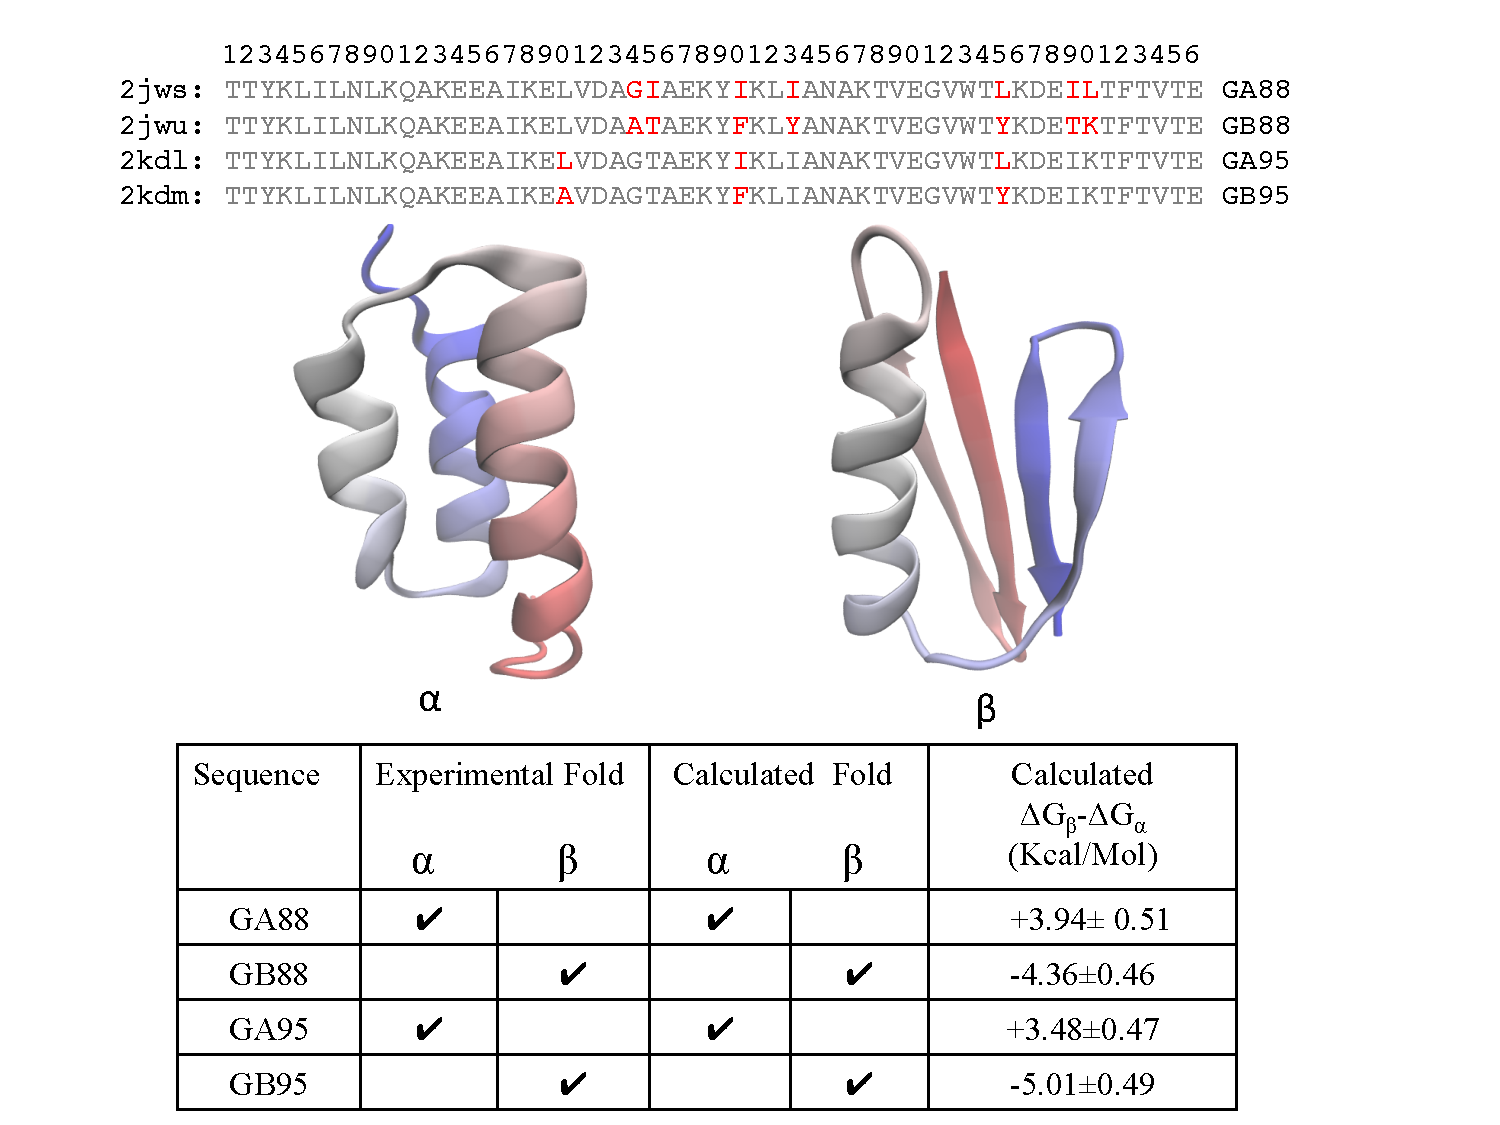
\includegraphics[width=3.5 in,height=4 in]{orban.pdf}
\label{fig:orban}
\caption{Confinement method correctly predicts the structural preferences of six chameleon
sequences. (A) The six sequences used in this study. (B) Each sequence adopts either a Protein
G-like fold (denoted GB) or a three-helix bundle fold (denoted GA). The relative free energies of
the two folds are reported for each sequence.}
\end{figure}

\begin{figure}
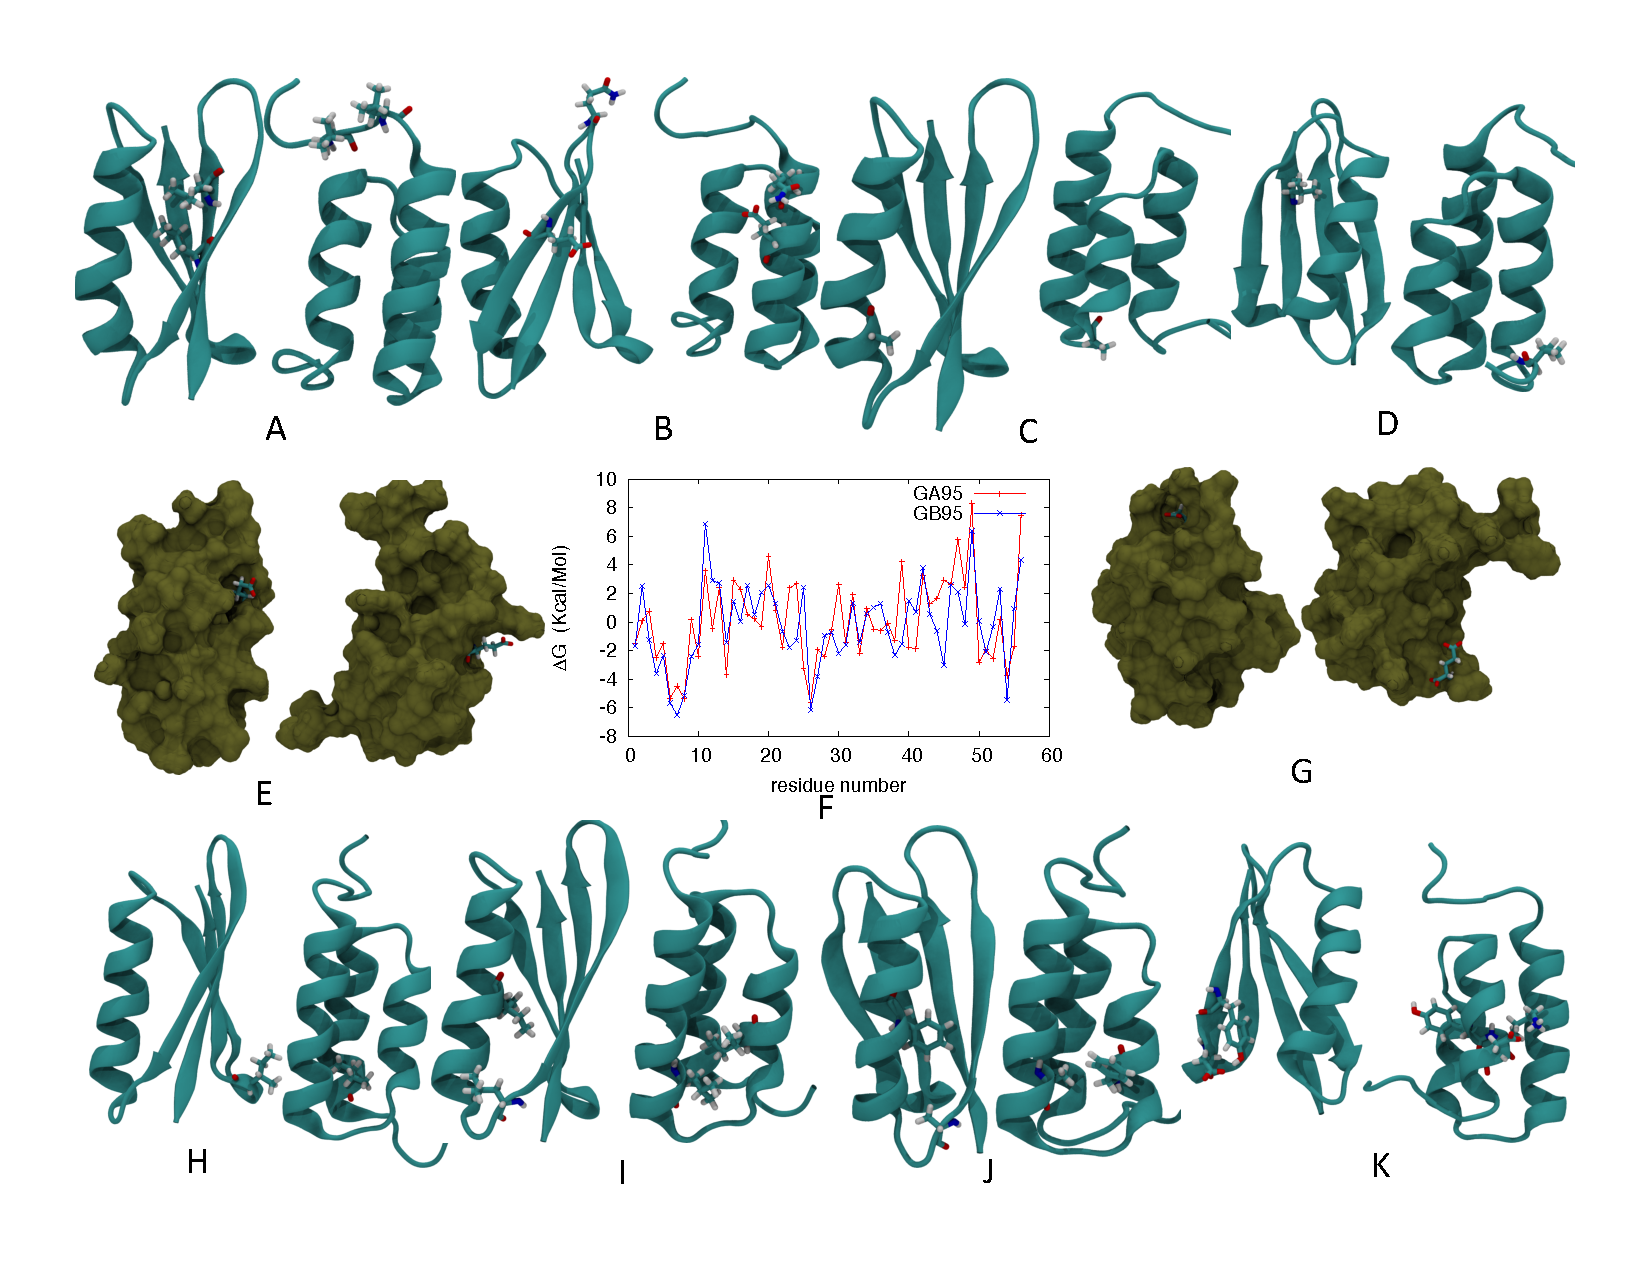
\includegraphics[width=6.4 in,height=5.3 in]{orban_full.pdf}
\label{fig:orban_full}
\caption{Sidechain orientation of some important residues which stabilize/destabilize either of the $4 \beta + \alpha$ or $3 \alpha$ conformation.
The details are in Table~\ref{table:orban_perresidue} and the main text.  
A. Leu-7.
B. Gln-11 has H-bond with Glu-15 in $3 \alpha$, which is absent in $4 \beta + \alpha$
C. Ala-26
D. Val-54.
E. Glu-14.
F. plot of free energy difference for GA95 and GB95 sequence. Positive peak stabilize $3 \alpha$ form and negative peak 
stabilize $4 \beta + \alpha$. 
G. Glu-56 .
H. sidechain orientation of Hydrophic Ile-49, along with Leu-20 and Ile-30 with GA95 sequence
I. sidechain orientation of Hydrophic Ile-49, along with Ala-20 and Phe-30 with GB95 sequence
J. Tyr-45 forms H-bond with Asp-47 with GB95 sequence and $4 \beta + \alpha$ conformation
K. No H-bond possible between Leu-45 and Asp-47 with GB95 sequence and $4 \beta + \alpha$ conformation .}  
\end{figure}


\subsection{The confinement method correctly identifies the most native-like predictions from a
subset of CASP predictions}

This method is particularly well suited to pick out the native/native like structure from misfolded or decoys. We have
tested this using different models from CASP (critical assessment of structure
prediction). CASP is a blind test in which different groups world wide apply their
methods to predict the 3D structure of proteins given their sequence. This is done with a strict 3
week limit on each target (3 day for servers) and each group is allowed to submit 5 possible
structures (ranked from best to worst). In our role as assessors during the CASP8 and CASP9 \cite{MacCallum2011}
competition we observed no correlation at all between the ordering of structures submited by the
groups and the real ranking compared to an experimental model \cite{Kryshtafovych2011}. The
consequences of this goes beyond
those five structures; the deeper meaning is that groups producing ensembles of structures are
generating structures that are better than the ones they submit, but they do not know about it. In
fact, when querrying different groups after the results were known, most groups agree that this is
the case. Beyond the CASP problem, this reflects on the modelers ability to correctly rank order
models in many different environments, such as structures for drug design leads or designing more
stable proteins or peptide mimetics such as peptoids. One of the main culprits of this lack of
accuracy is the fact that ranking is often done via a potential energy function, which in many cases
lacks an entropy component. Other initiatives including knowledge based potentials do use some sort
of free energy to rank order, but its accuracy is not enough. Our method provides a physics based
solution to this problem. We have tried two experiments centered on CASP. First we tried to rank
order some structures from the previous CASP9 experiment. We have tested different options for that purpose.
First, we rank order submitions from same group and then from different groups. Our second test was 
to check whether this method can do better quality assessment/metaprediction than the best group in that catagory in CASP9. 
In both methods, our ranking is determined as a free energy measure,
and it is compared with the ranking given by a geometrical comparison between native and submitted
models called GDT\_TS (Global distance test score \cite{Zemla2003}). 
GDT\_TS represents the average percentage of residues that are in close proximity in two
structures optimally superimposed using four different distance cutoffs (1, 2, 4 and 8 \AA).

We have chosen the inital models on which to test the methods based on server groups that have
traditionally done good in past CASP events. There is a high correlation between the structures that
are chosen for this method and its predictive accuracy. In particular, when GDT\_TS scores are below
50, it is difficult for us to say anything about the models. Our approach is simple, for every
subset of structures we choose, we use the confinement method in a pairwise procedure, and then rank
the structures. In all cases, we have also calculated the free energy with respect to the native
structure to check the stability of the models.
However, this step is not needed if we just want to rank order.

\subsubsection{The confinement method can rank different models generated by the same methodology and distinguish the native structure}

The question that we want to answer here is whether we can rank models that have been generated with
the same methodology. In all cases, we have calculated the free energy
difference between the native structure and the submitted models as well. 
%Identifying the native state from a set of models is a very easy test, that most metapredictors
%already handle correctly, but it is also a first proof of principle. 
First we choose a protein BVU3908 from Bacteroides vulgatus whose PDB id and CASP target code are
2L01 and T0559 respectively. The native structure of this 69 residue protein was solved using NMR.
The best predictor group for this target was "BAKER-ROSETTASERVER".
We initially checked similarity between the models submitted by "BAKER-ROSETTASERVER" and discarded two of them from the 
analysis on the basis of being too similar to some of the other models. The GDT\_TS score and rmsd
values as shown in Figure~\ref{fig:T0559} indicate that model 1 was predicted correctly, 
whereas the order of model 3 and 5 was wrong. The main difference
between model 3 and the rest of the models is that the orientation of the first alpha helix of model
3 is \Alberto{opposite??}.
On the other hand, as shown in Figure~\ref{fig:T0559} the confine and release method not only can differentiate the native 
structure from the submitted models, the ranking also correlates perfectly with the GDT\_TS score.  

To further test the method we have taken the example of protein BT2368 from Bacteroides thetaiotaomicron. The PDB id of this 
74 amino acid residue protein is 2L02 and CASP target code is T0560. We have compared the free energy difference between 
the native structure and the two of the five submitted models from the group "Splicer". The remaining three models are discarded as 
again they are similar to the rest of the models. The comparison of GDT\_TS score as shown in 
Figure~\ref{fig:T0560} and published in the final CASP result is only for models with residues 3 to 66. In order to keep
consistency, we have also done our analysis with models and crystal structure consisting residues 3 to 66. As expected,
the native state is identified correctly, and the two other models are ranked in the correct order in accordance with the GDT\_TS score.   

\subsubsection{The confinement method can rank models generated by different methods}

Our next test was between models that are produced with different methodologies. We do this by
looking at some of the best CASP submissions from different research groups. 
For this purpose we have chosen the x-ray crystallographic structure of 
fas apoptosis inhibitory protein molecule whose pdb id and CASP target codes are 3MX7 and T0540 respectively.
This protein contain 90 amino acid residues with 8 beta strands. We have chosen best models from groups
"LTB" and "Mufold" for our analysis, which are labelled as Model 1 and Model 2 in Figure~\ref{fig:T0540}.
As presented in  Figure~\ref{fig:T0540} we found that this method is able to correctly order the models which matches
with the GDT\_TS score. 

\subsubsection{Per residue free energy calculation identifies the residues that are responsible for
differences between two conformations}

We used one of the CASP targets (pdb id=2KWY, casp id=T0569) to study the per residue contribution
between this NMR structure and the best CASP9 predicted model (from the 'Mufold' group, GDT\_TS=78).
Visualization upon superimposition of two structures reveals that
the difference between the two structure is at the region consist of residues 48 to 65, where model1 is much more disordered compare to the
native structure(see Figure~\ref{fig:T0569}). Other regions look similar for both the cases with of model1 is within 2.6 \AA backbone
rmsd value of the native structure. We found that, the confinement method can still differentiate between the native structure and 
the generated model. We have also calculated the per residue free energy with a aim that this can identify the residue which are responsible
for such free enerfy difference. The per residue free energy decomposition is shown in  Figure~\ref{fig:T0569_per_residue}(A). We indeed 
found that two hydrophobic residues Val-59 and Ile-61 are oriented towards the solvent in the protein 
surface in the generated model (Figure~\ref{fig:T0569_per_residue}(B). This the region, where there is a beta sheet in the original crystal structure, which is absent in the 
model. Interestinlgy, some regions are more stable in the generated model. A close inspection
reveals that 
the hydrophilic Glu in position 67 is completely exposed to the protein surface and solvent in the best model, whereas it is partially exposed in the 
crystal (Figure~\ref{fig:T0569_per_residue}(C)). The peak at position 76 is due to the H-bond between Lys-76 and Asp-11, 
which is absent in the original crystalographic structure (Figure~\ref{fig:T0569_per_residue}(D)). 
   
\subsubsection{Failures in the confinement method}

Despite the great success in most of the studied systems, we found a few failures, specially when
the GDT scores of the compared structures are
very close. We have found this for an engineered protein from Asr4154 protein (PDB ID: 2L09 and CASP Target T0538).
This protein contains 54 amino acid residues with three alpha helixes and two very short beta
strands. 
The model that is closest to the native structure was generated by the group PconsR with a GDT\_TS value of 96.23.
We have also considered one model from group "Shell" (GDT\_TS = 90.09) and "FOLDIT" (GDT\_TS = 86.32) for our analysis along with
the native crystal struture (RMSD values between 1.6 and 2.0\AA \Alberto{from native, right?all
atom? CA?}). The models from PconsR, Shell and FOLDIT are labelled as model 1, model 2 and model 3 
respectively in Figure~\ref{fig:T0538}. As seen in Figure~\ref{fig:T0538}, one can find that the 
model from PconsR has lowest free energy value, making it a more stable structure. Although ranking of the other models
remains consistent, model 1 is predicted to be more stable than the
crystal structure. To rationalize this, we have decomposed the total free energy into the per
residue components. The results show us that despite the small variation at the backbone level (as
shown by high GDT\_TS scores and low RMSDs), the sidechains are oriented in very different ways,
giving raise to large differences in the stabilization of certain residues.
In particular, some of the differences arise from different salt bridge patterns (Arg-32 with Glu-35
and Glu-28 with Lys-24
in crystal versus Arg-32 with Glu-28 in model 1) and certain flexible polar residues exposed to the
surface (Lys-24 in model 1, which has an entropic gain from not forming a salt bridge and is
stabilized by interactions with the solvent). This is summarized in Figure~\ref{fig:T0538compare}(A) 
Similar patterns arise in other places of the protein (see Figure ~\ref{fig:T0538compare}(B)), where
the salt bridge between Arg-26 and Glu-50 is absent in model 1 and is further \Alberto{stabilized?} by Phe-51
having a very different conformation that in the crystal structure.
All in all, this unexpected result just shows us that this method is sensitive to local interactions
such as those happening from side chain reorientation. At the same time, the results explained in
past sections showed that for larger changes the accuracy of the method is very high.

\subsubsection{What can we say about low resolution models?}

So far we have seen that the method is good at predicting preferences when the structures are not
very close to each other, how far from native can we go? In this section we want to explore what
happens when we use the method to describe low quality models. We use one of the CASP targets (pdb
id = 2KJX, CASP id = T0531) .
We mentioned earlier that our predictive abilities are greatly decreased with low model qualities. 
Comparing low qualitive models between themselves is not very informative,
    however, comparing all of them to a native/native like structure, allows to rank order this
structures. 
In order to test this hypothesis we performed another test with target T0531 of CASP9, in which we compared the crystal 
structure to five models from the MUFOLD server. Pdb id of this extracellular domain of the jumping translocation 
breakpoint protein is 2KJX and CASP target code is T0531.
Looking at Figure~\ref{fig:T0531} shows: 1.) native is correctly
identified as expected and 2.) Surprisingly there is a high level of correlation between the GDT
ranking and the free energy ranking for model 1 and model 3, the rest three structures with GDT\_TS score less than  35  are ordered
incorrectly. It is worth to note that models 2 and 3 have the same GDT and very different free
energies, meaning that the actual ordering could change a lot \cite{Perez2012}. It is encouraging that at least
the method can pick out the best model even though it is got a low GDT score: 44.  

%\subsubsection{Difficulty in CASP Experiments}

%It is often difficult to model CASP targets using the confinement and release method. There are many cases,
%where the sequence of a particular target is trimmed during actual result presentation. This is illustrated
%with the crystal structure of the leucine zipper domain of cGMP dependent protein kinase I (pdb id: 3NMD
%and CASP9 code: T0605) as shown in Figure~\ref{fig:T0605}. The actual CASP 9 target consisted of 72 amino acid residues, but
%as only 18-66 amino acid residues could be detected in actual crystal structure of this protein, the final result was trimmed 
%with respect to that crystal structure with 49 amino acid residues which consist of a single alpha helix. The amino acid residues 18 and 66 are shown in
%three models submitted by the group "Baker". It is important to note that blind prediction of model ranking on the basis of free energy can be hugely 
%affected in such scenario as the only major difference between those models are the trimmed parts, specially the region consisting residues 1-18.    


\subsubsection{Can the confinement method perform better quality assessment in protein structure prediction?}
A part of the CASP experiment is dedicated to the assessment of the quality of predicted models \cite{Kryshtafovych2011}. 
Most of the top performing groups in this category use consensus approaches for quality assessment \cite{Wang2011}.
A review of CASP9 quality assessment also pointed out that the methods which are based on clustering
techniques perform
much better compared to those methods which are based on analysis of individual models \cite{Kryshtafovych2011}. 
In this background we try to answer, whether the confinement method can do better quality assessment
compared to the best performing
group (MUFOLD-WQA) in this catagory. In CASP9, the overall reliability of models in quality assessment (QA) was accepted in a mode known as
QMODE 1. Here, predictors were asked to score each model on a scale from 0 to 1, with higher values corresponding to better models \cite{Kryshtafovych2011}. 
We have again picked up the CASP taget T0538 to answer this question. We have chosen Model 3 submitted by PconsR (GDT\_TS = 96, QMODE 1 = 0.5434) 
and model 5 from the MULTICOM-NOVEL ( GDT\_TS = 83, QMODE 1 = 0.5865). Both are server predicted models and they were further used for quality assessment 
by the group MUFOLD-WQA \cite{Wang2011}. It is important to note that the model from PconsR was the most accurate predicted model for this 
target and the model from MULTICOM-NOVEL was predicted as best by the quality assessment experiments of MUFOLD-WQA. Also, 
the QMODE 1 value presented here is from the group MUFOLD-WQA. 
Our free energy analysis predict that the model from Pconsr is indeed better than the model from 
MULTICOM-NOVEL $(\Delta \Delta G (Model\_Pconsr - Model\_MULTICOM-NOVEL = -3.9 Kcal/Mol)$, which   
matches well with the GDT\_TS score. On the other hand the MUFOLD-WQA predicted the ranking in the reverse order. 

We have also carried out a similar type of analysis for the case of Target 560 from the CASP9 experiment. For that 
we have chosen the model 1 from the group PconsR (GDT\_TS = 94, QMODE 1 = 0.5178), Bilab\-Enable (GDT\_TS = 87, QMODE 1 = 0.5344) 
and Multicom\_Refine (GDT\_TS = 74, QMODE 1 = 0.4770). If, one wants to rank order with respect to the GDT\_TS values, the model from 
PconsR is the best predicted model, but according to the QA assessment by MUFOLD-WQA, the model from Bilab-Enable was found to be best predicted model. 
All the QMODE 1 values are from MUFOLD\-WQA. In CASP 9, the sequence of 74 residues were given to predict the structure and for 
quality assessment, whereas during GDT\_TS analysis only residues 3-66 were considered. When we considered the full 74 amino acid 
residues, the free energy calculated were $(\Delta \Delta G (Model\_Pconsr - Model\_Bilab\-Enable = 3.3 Kcal/Mol)$ and 
$(\Delta \Delta G (Model\_Pconsr - Model\_Multicom\_Refine = -30.0 Kcal/Mol)$ \Alberto{-30 sounds
huge!} which 
support the QA assessment by MUFOLD-WQA. On the other hand, if we calculate the same free energy with the trimmed version of the protein 
(with residues 3-66), the values of the free energy difference become -1.7 and -31.1 Kcal/Mol respectively, which support the GDT\_TS score. 
The summary of this whole observation is presented in Table~\ref{table:560QA}.
There is no doubt that the consensus approach can predict the model quality in a faster manner. But
we expect that the confinement
method can predict the model quality in a relatively expensive but much more accurate way.

\begin{table}
\label{table:560QA}
\begin{center}
\begin{tabular}{| l | l | l | l | l |}
\hline
Model            &  $\Delta \Delta G$ (1-74)  & $\Delta \Delta G$ (3-66) &    GDT\_TS    & QMODE 1  \\ \hline
PconsR           &         0.0                &      0.0                 &    94         &  0.5178   \\ \hline
Bilab\-Enable     &        -3.3                &      1.7                 &    87         &  0.5344   \\ \hline
Multicom\_Refine &        30.0                &     31.1                 &    74         &  0.4770   \\ \hline
\end{tabular}
\end{center}
\caption{Comparison of quality assessment by the group MUFOLD\-WQA and the confinement method of the CASP9 target 560 (pdb id: 2L02). 
The GDT\_TS score obtained from CASP9 website, was based on the trimmed model containing residue 3-66, whereas, the QMODE 1 values are from
quality assessment by the group MUFOLD\-WQA and based on residues 1-74.}
\end{table}  


\section{Conclusion}


The last 50 years represent our effort to understand what the native state of a protein
    looks like by using theoretical methods. Experimental evidence coming from NMR and x-ray
    cristallography remain so far the only real ways to solve the structure of the native state.
    However, this methods are expensive and slow. Theoretical methods on the other hand are cheaper,
    but despite improvement still have a long way to go. Often this computational pipelines produce
    ensembles of diverse structures and identifying which structure is more native like is still a
    problem. Here we have shown how the application of the confinement method can help identify
    native like states. The high success rate balances with the computational expense. However, with
    GPU technology and the rate at which computers improve, this computational expense is becoming
less of a bottle neck.
We foresee great potential for this methodology for two reasons: independence from a reaction
coordinate (just need start and end state) and avility to decompose the free energies on a per
residues basis. This last point can be very useful in protein design. Finally, we have presented
data for structure comparison of proteins, but we are currently exploring the possibility of
using this methodology for getting free energies of ligand-protein binding. 
\Alberto{Do we mention this in the text? too technical for conclusions:
There is another issue, which is normal mode
analysis calculations are Oh(N**3) and require large amounts of memory, effectively limiting the
size of the systems under study. In most cases quasiharmonic analysis.   
}

\section{Method}

The confinement method has been described in details in ref. by Tyka et.al. \cite{Tyka2006} and 
Cecchini et. al. \cite{Cecchini2009}. The basic approach of the confinement approach is the same in both
these papers. However, there are some technical differences. Here we briefly describe the procedure
to compute free energy $\Delta G_{AB}$ between two conformations A and B of a protein. The basic
idea to compute the free energy between conformations A and B is to perform a thermodynamic cycle: 

\begin{enumerate}

\item  Minimization of A and B. These minimized conformations (A* and B*) 
       are the reference conformation of that state. During this minimization the backbone is kept
       restrained to the original position to avoid large conformational changes.

   \item  The free energy of confining the ensemble (A or B) to a microstate (A* or B*) is
       calculated. This is done by gradually applying larger and larger
       harmonic restraints on all the atoms of the biomolecule. This is done by running 21 molecular dynamics simulation 
       (20 ns long each), where the harmonic restraint force constant was scaled from 0.00005
       \Alberto{units??}
       (mostly free) to 81.92 (frozen in one microstate). In this final restrained state, the
       rotational contribution to the free energy is frozen out
       and the only remaining contribution is the vibrational part. The free energy for this step is
       estimated from the fluctuations around
       the reference structure using a numerical
       approach developed by Tyka et. al. \cite{Tyka2006}. The confinement free energy calculated in
       this way is recorded as 
       $\Delta G_{A,A*}$ and $\Delta G_{B,B*}$ as shown in Figure~\ref{fig:method}.     

\item  Finally the thermodynamic cycle is closed by calculating the free energy between the final
       restrained state A* and B* using normal mode analysis or quasiharmonic analysis. The free energy calculated in 
       this way is shown as $\Delta G_{A*,B*}$ in Figure~\ref{fig:method}.

\item  The full free energy, $\Delta G_{A,B}$ between the two state A and B is calculated using the equation 
       $\Delta G_{A,B}$ = $\Delta G_{A,A*}$ - $\Delta G_{B,B*}$ + $\Delta G_{A*,B*}$  

\end{enumerate}

 All calculations where performed with the amber 11 suit of programs in combination with ff99SB and GB/SA implicit solvent. Interestingly, we extend the
method for calculation of per residue free energy in an approximate way. For this purpose, the confinement energy, 
$\Delta G_{A,A*}$ and $\Delta G_{B,B*}$ of each residue is calculated in the usual numerical way as described above. The
internal energy of each residue is calculated using the decomp module of amber from the final restrained trajectory. We 
call this method approximate as we ignore the contribution from the normal mode or quasiharmonic analysis. 
However, this contrbution to the total free energy is much smaller (less than $1.0
Kcal/Mol$\Alberto{that sounds huge, i would say what percent of error we stimate, I think it was
lower than 1kcal/mol}), which allow us to 
study the mechanistic details of conformational preference of each residue.      

%There are two big bottlenecks in this calculation. The first has to do with the amount of
%simulations that have to be performed to confine the ensemble of conformations close to a microstate
%into a single microstate, the second bottleneck has to do with the size of the system in the normal
%mode calculation. We have tackled the first issue by using GPU (Graphical Processing Unit) technology as opposed to the classical
%CPUs, which gives us a two order of magnitude boost in computational efficiency. Normal mode
%analysis calculations are Oh(N**3) and require large amounts of memory, effectively limiting the
%size of the systems under study. Where as this can be overcome by larger memory machines, these are
%often not available, and so we propose an alternative by using quasiharmonic analysis. This is still
%an Oh(N**3) problem, but we now the motions of atoms are already determined in trajectories, and so
%we can choose to do quasiharmonic analysis excluding hydrogens, which will reduce the number of
%atoms N to almost N/2. This means that we can use this method for systems twice as large.


\begin{figure}
\begin{center}
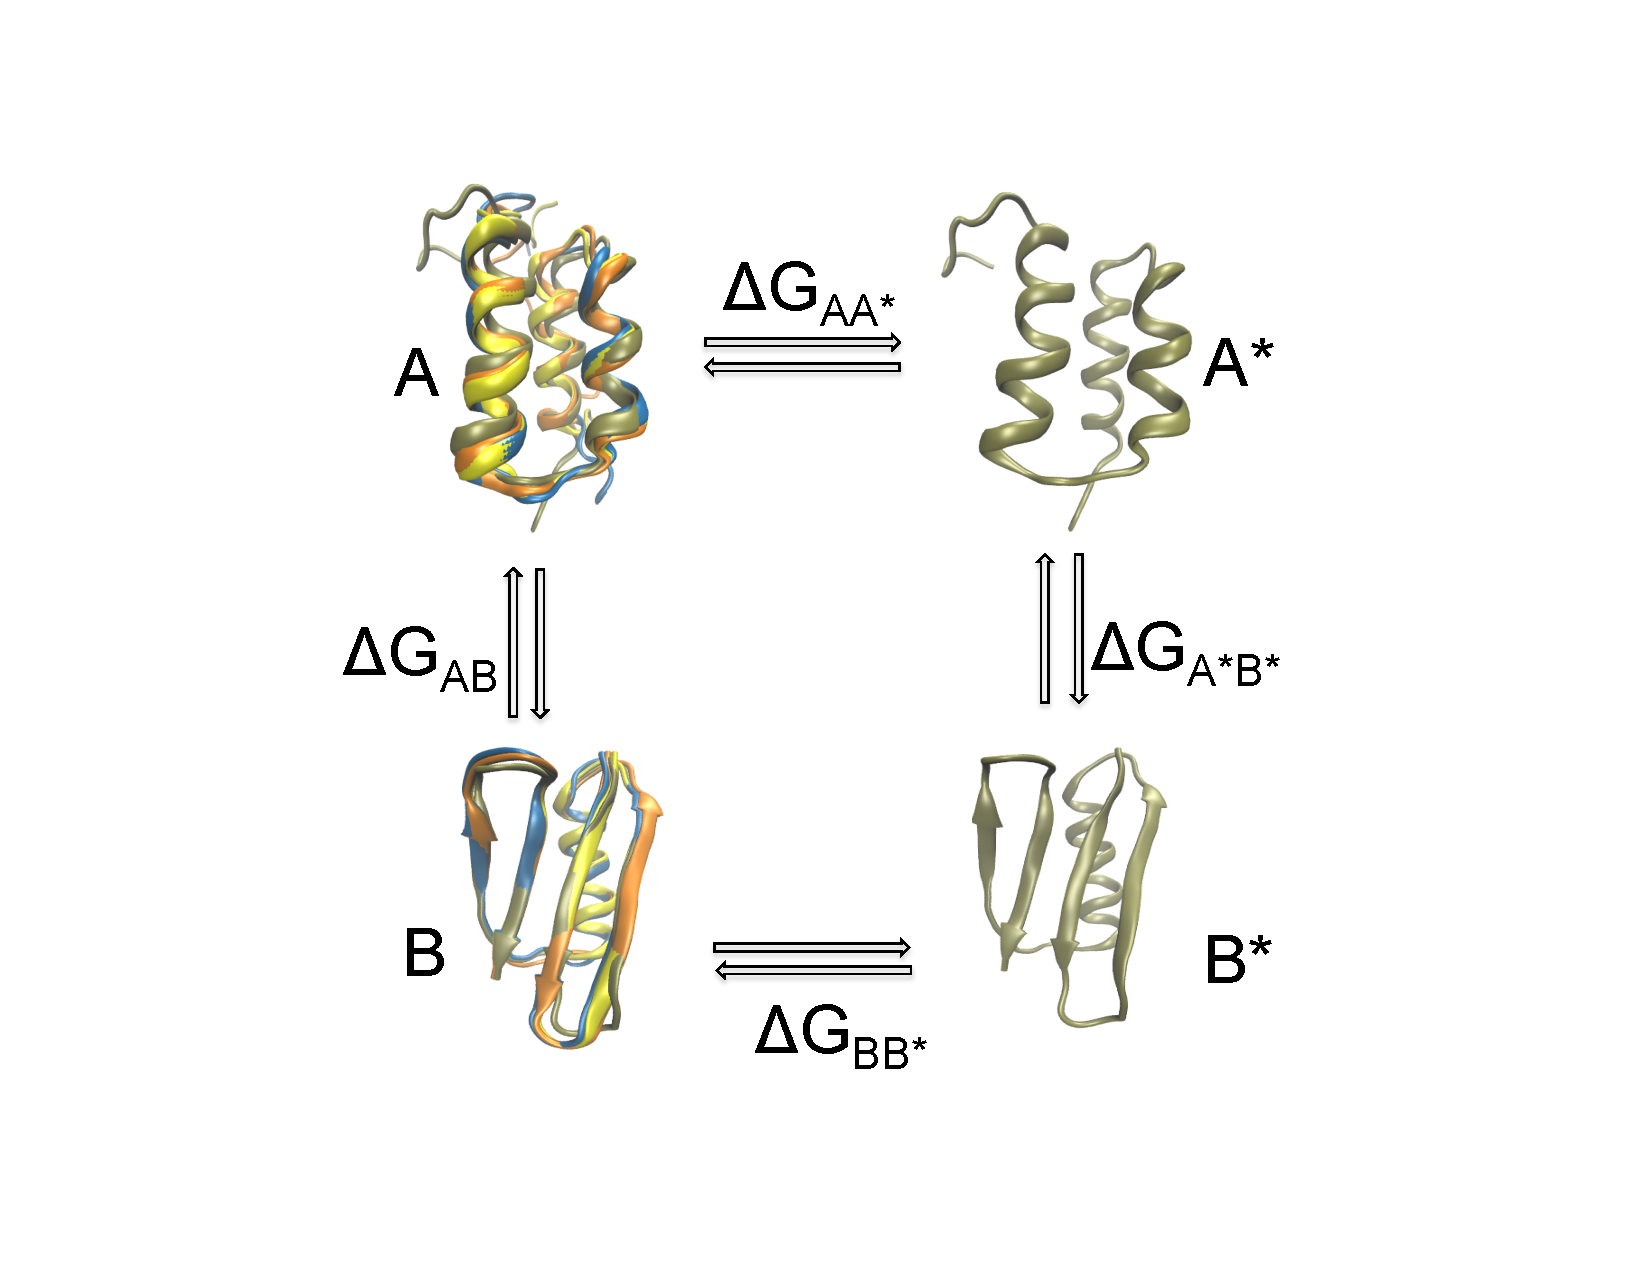
\includegraphics[width=3.5 in,height=3.5 in]{method.pdf}
\end{center}
\caption{Graphical representation of the thermodynamic cycle involving confinement method.}
\label{fig:method}
\end{figure}

%\begin{figure}
%\begin{center}
%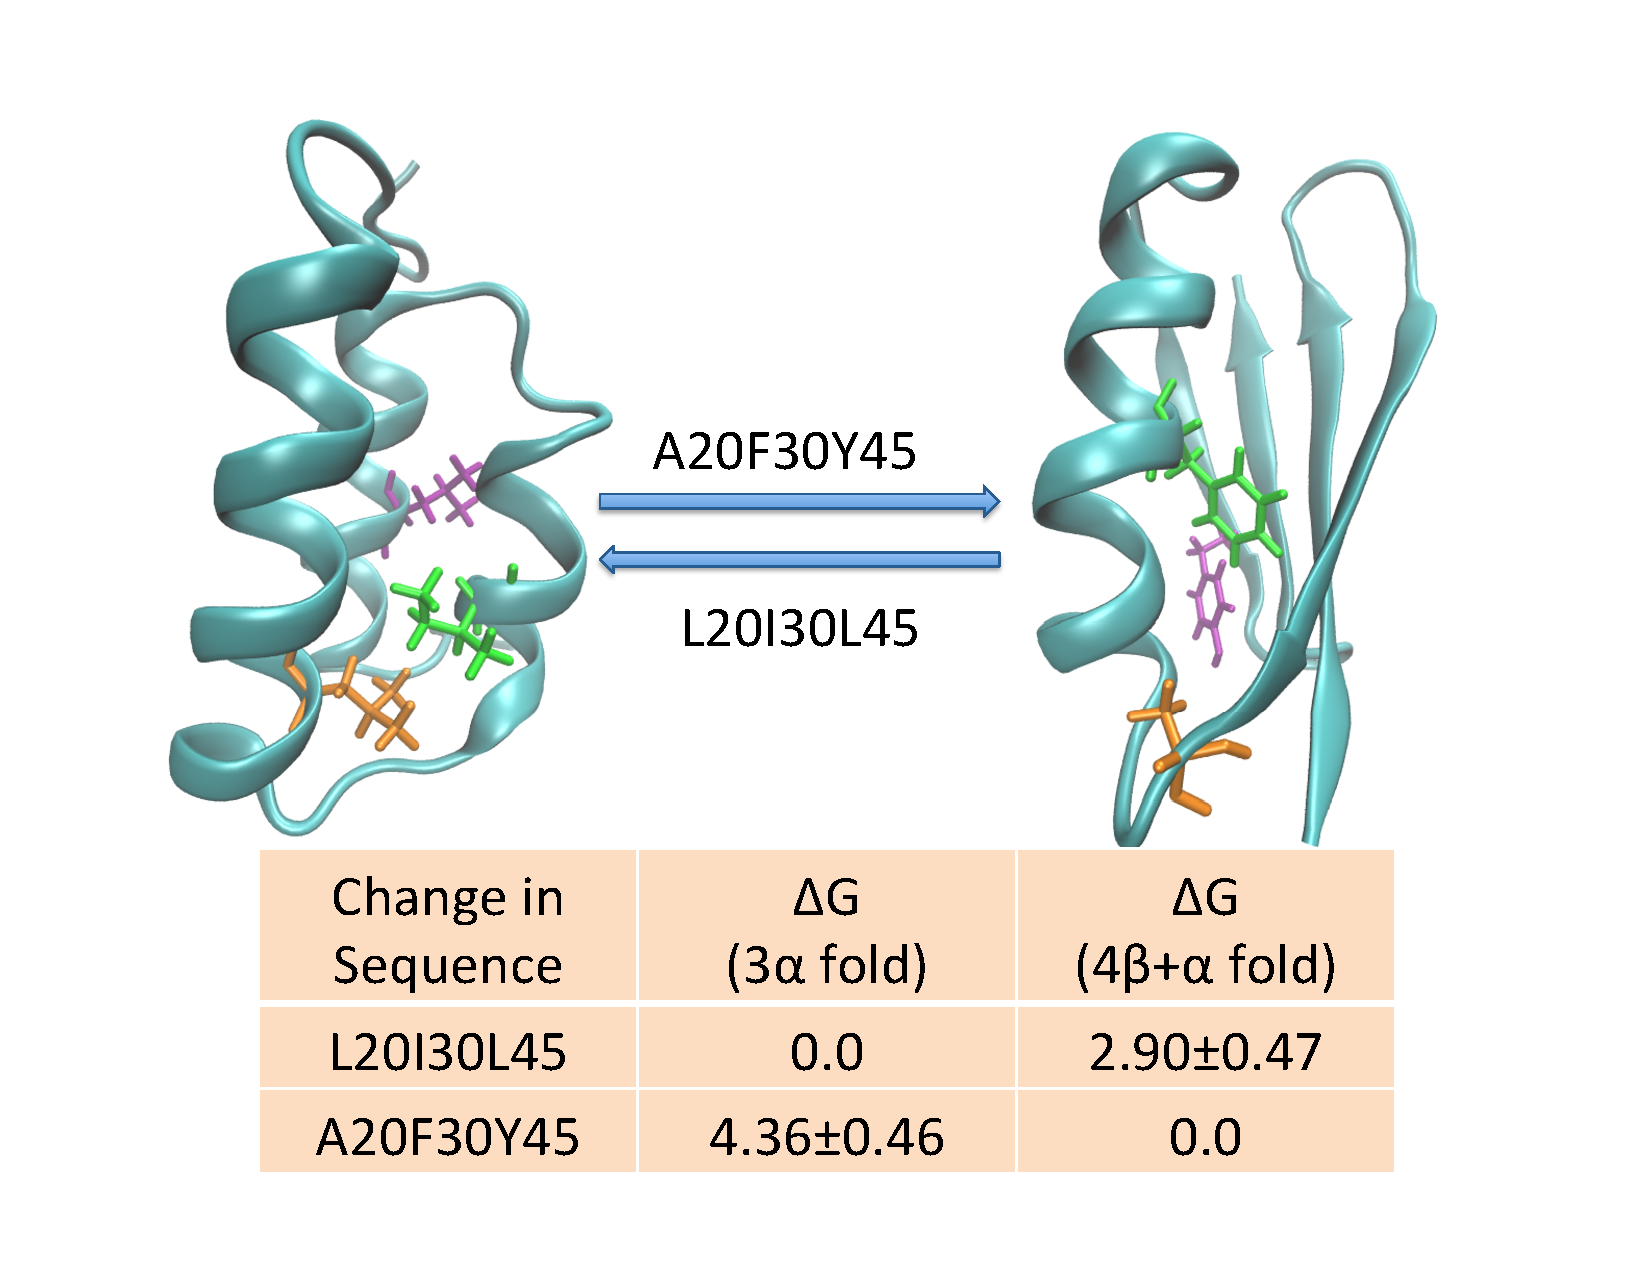
\includegraphics[width=3.5 in,height=3.0 in]{G95.pdf}
%\end{center}
%\caption{Two protein with 95 \% similar sequence but different folds}
%\label{fig:G95}
%\end{figure}

\begin{figure}
\begin{center}
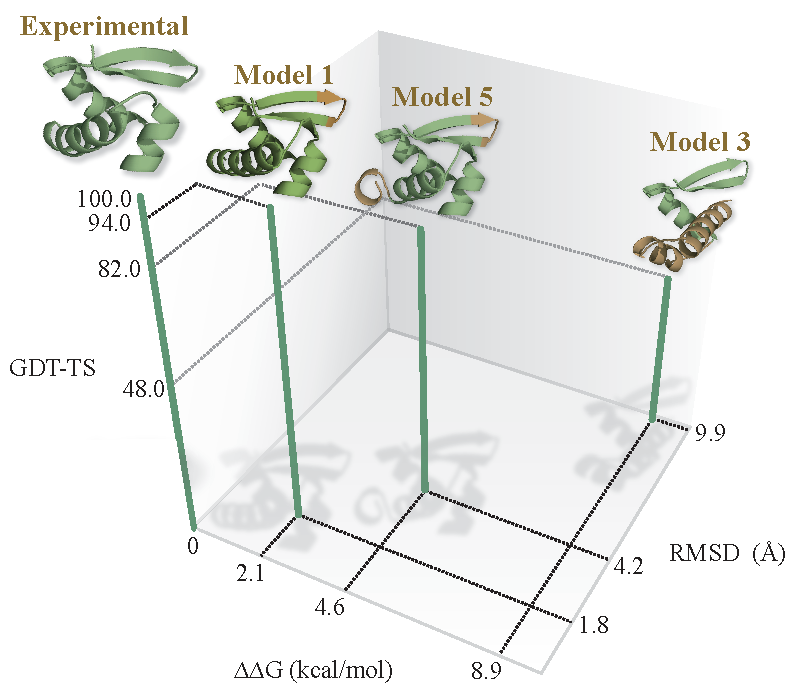
\includegraphics[width=3.8 in,height=3.0 in]{T0559.pdf}
\end{center}
\caption{The native and three submitted model structure, along with their GDT\_TS, RMSD and relative Free energy values 
of protein BVU3908 from Bacteroides vulgatus (PDB id: 2L01 and CASP code: T0559).}
\label{fig:T0559}
\end{figure}

\begin{figure}
\begin{center}
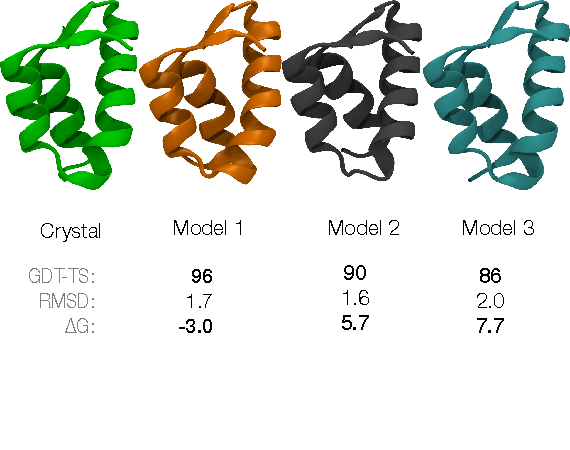
\includegraphics[width=3.8 in,height=3.0 in]{T0538.pdf}
\end{center}
\caption{The native and three model structure of engineered protein from Asr4154 protein (PDB ID: 2L09 and CASP code:T0538). The model 1,2 and 3 are
from the group PconsR, Shell and FOLDIT respectively.}
\label{fig:T0538}
\end{figure}

\begin{figure}
\begin{center}
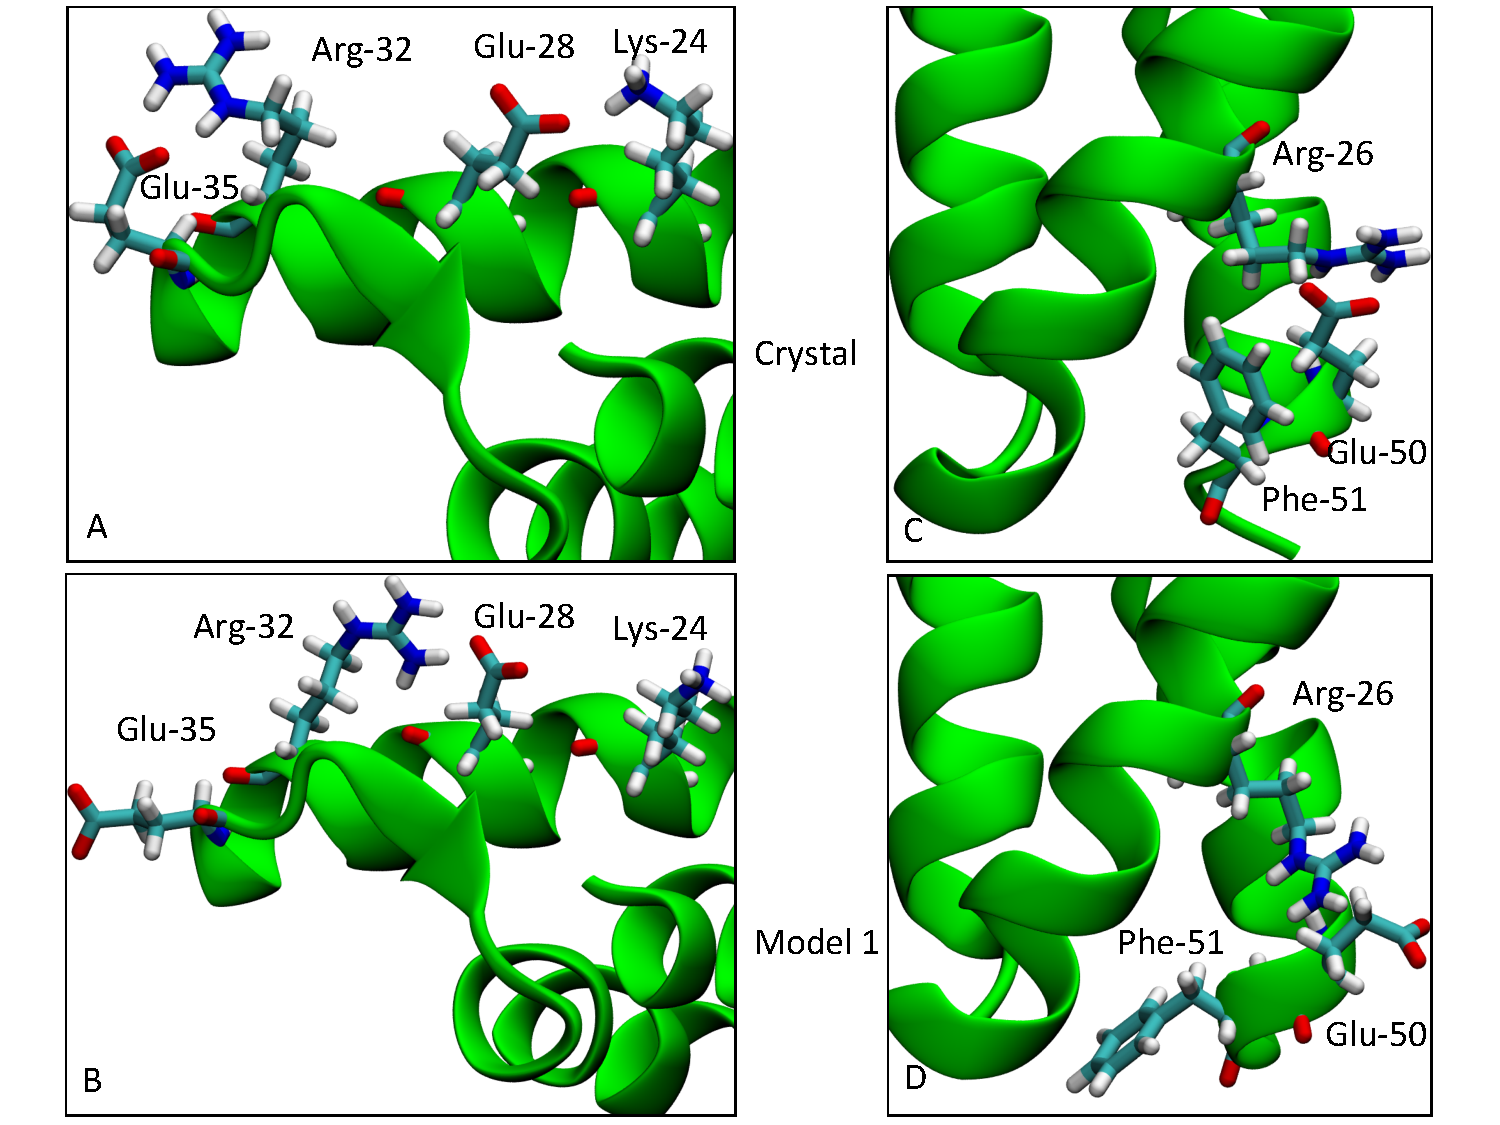
\includegraphics[width=4.9 in,height=4.0 in]{Target_538_compare.pdf}
\end{center}
\caption{Difference of the sidechain orientation between model 1 and crystallographic structure in Target-538.
A. The salt bridge between Glu-35 and Arg-32 in crystal structure. In model 1, this is compensated by H-bonding between 
Arg-32 and Glu-28. There is another salt bridge between Glu-28 and Lys-24.
B. Salt bridge between Arg-26 and Glu-50 in crystal structure. Orientation of Phe-51 is different in crystal than in model1.}
\label{fig:T0538compare}
\end{figure}


\begin{figure}
\begin{center}
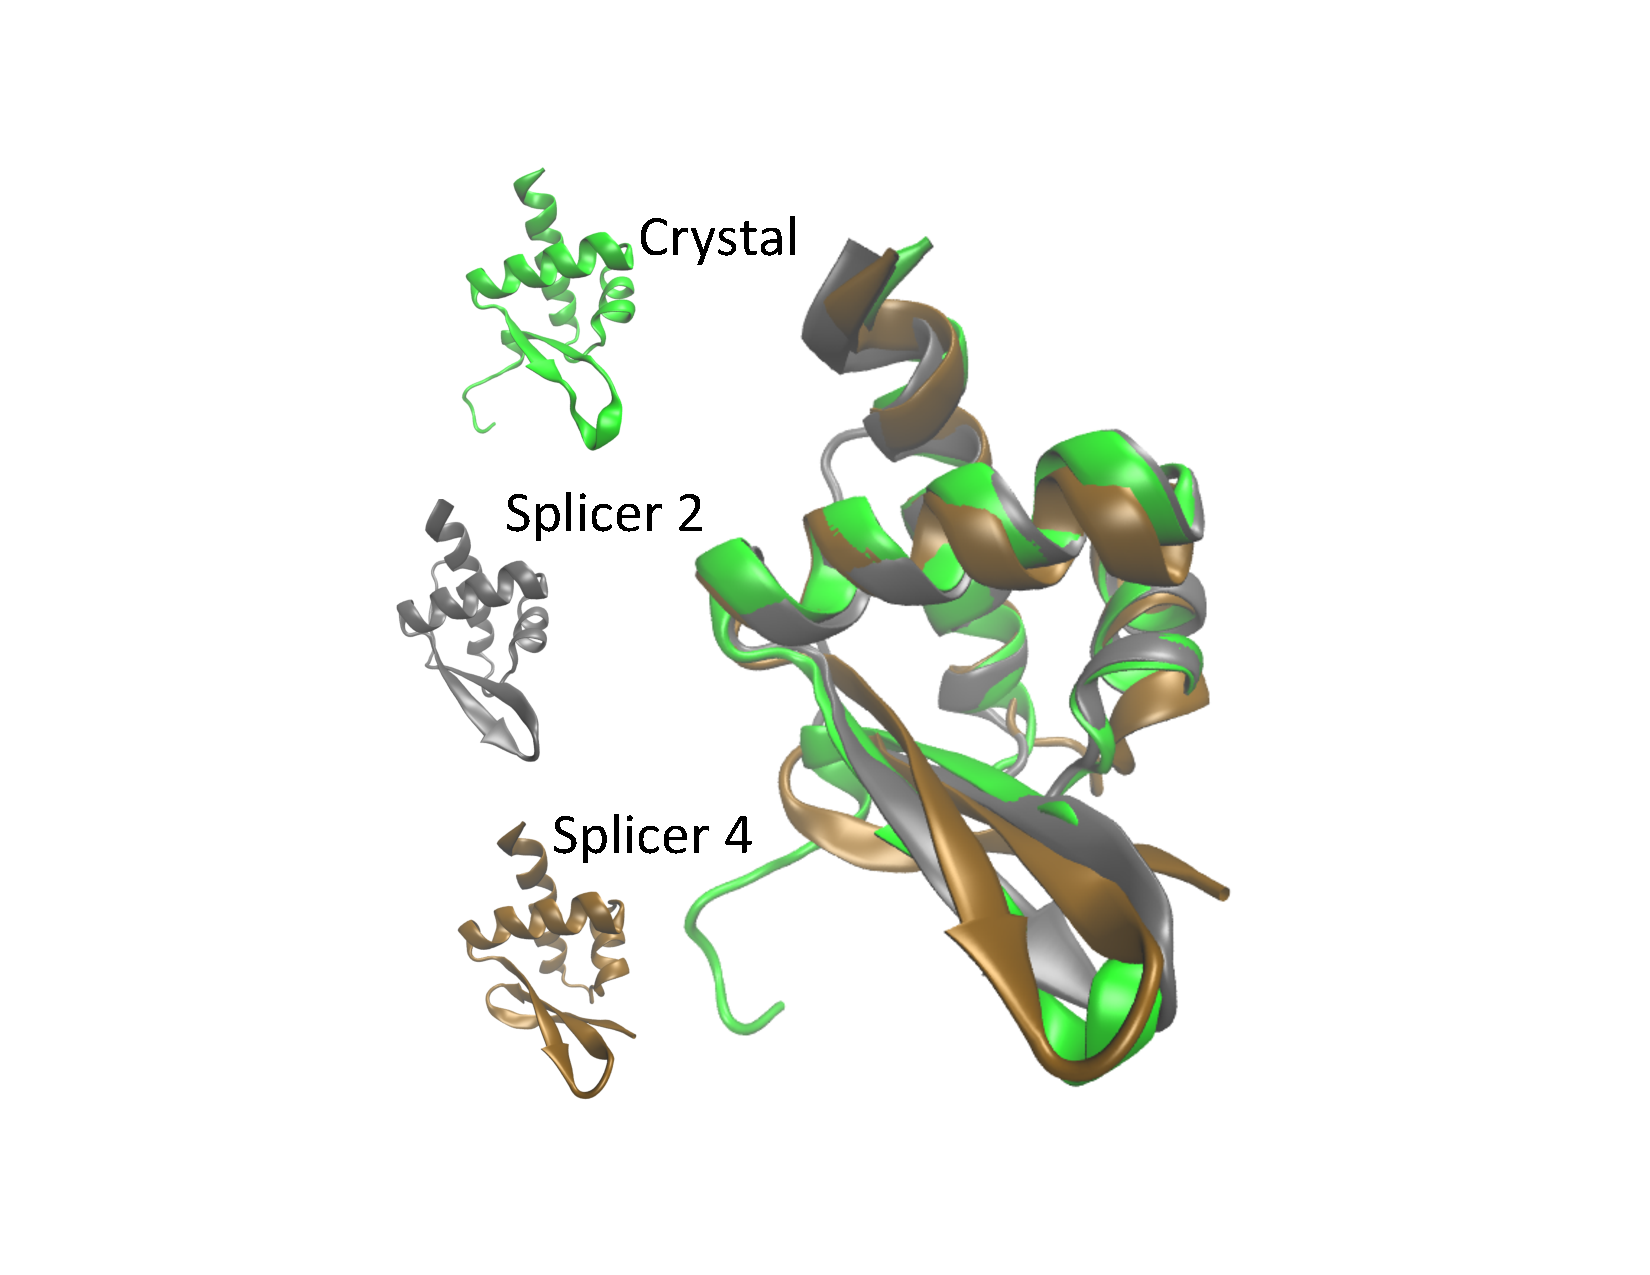
\includegraphics[width=3.5 in,height=3.0 in]{T0560.pdf}
\end{center}
\caption{Native and two model structure of protein BT2368 from Bacteroides thetaiotaomicron (pdb id: 2L02 and CASP code: T0560). The two models
were from the group "Splicer".}
\label{fig:T0560}
\end{figure}

\begin{figure}
\begin{center}
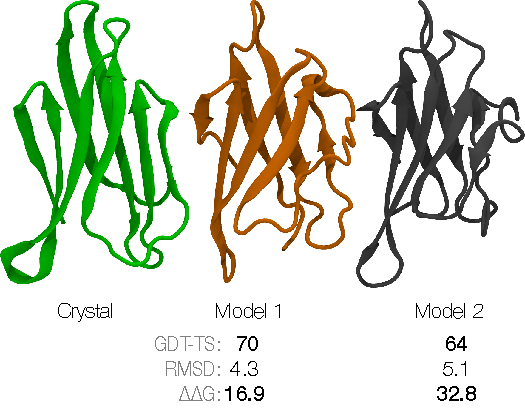
\includegraphics[width=3.5 in,height=3.0 in]{T0540.pdf}
\end{center}
\caption{X-ray crystallographic structure and two submitted models of fas apoptosis inhibitory protein (pdb id: 3MX7 and CASP code: T0540). 
Model 1 and Model 2 in this analysis were submitted by the group LTB and MUFOLD respectively.}
\label{fig:T0540}
\end{figure}

\begin{figure}
\begin{center}
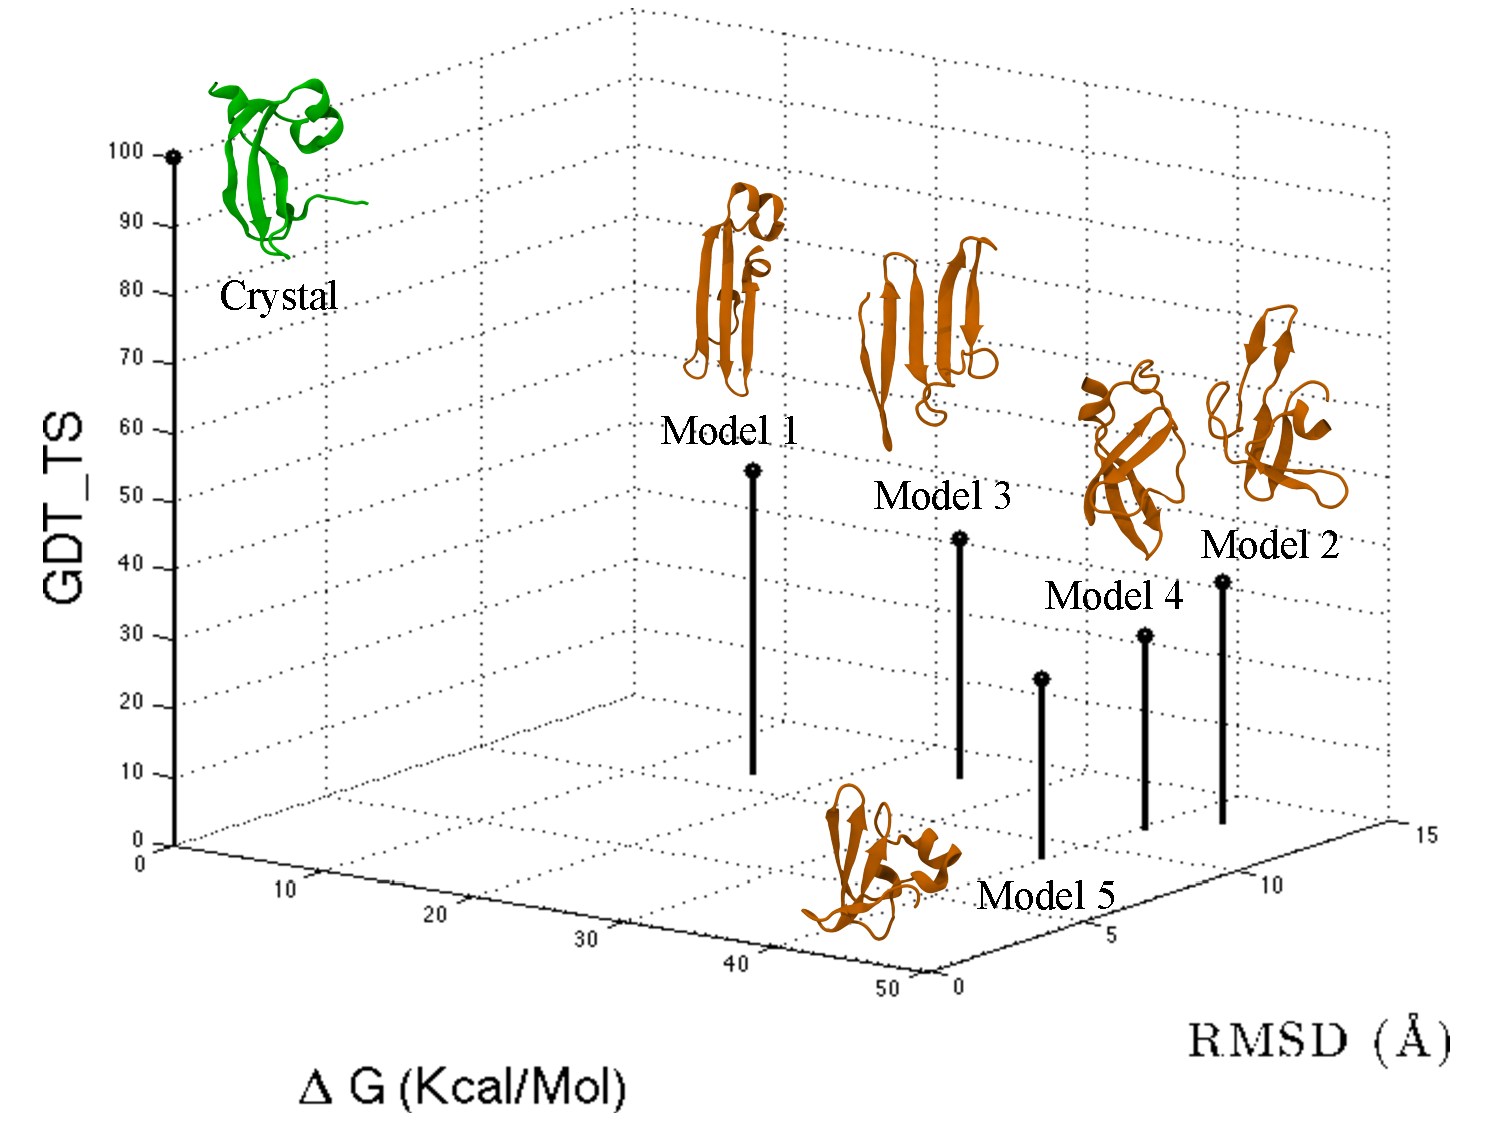
\includegraphics[width=3.5 in,height=5.7 in]{T0531.pdf}
\end{center}
\caption{The native structure and 5 models of extracellular domain of the jumping translocation
breakpoint protein (pdb id: 2KJX and the CASP code: T0531).}
\label{fig:T0531}
\end{figure}

\begin{figure}
\begin{center}
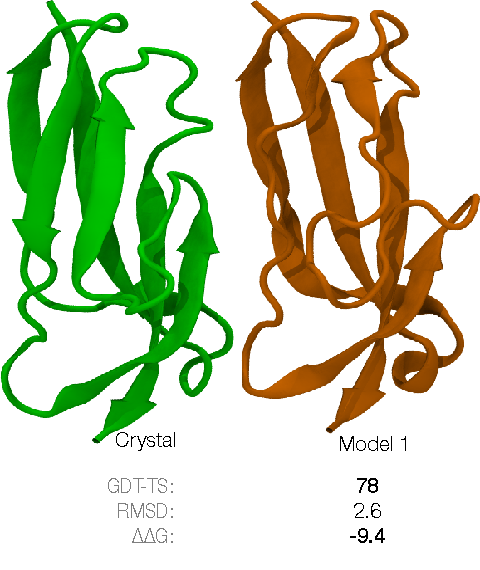
\includegraphics[width=3.2 in,height=3.8 in]{T0569.pdf}
\end{center}
\caption{Native and best model structure of a domain of adhesion exoprotein from Pediococcus pentosaceus (pdb id: 2KWY and CASP code: T0569).
The best model was from the group "Mufold".}
\label{fig:T0569}
\end{figure}

\begin{figure}
\begin{center}
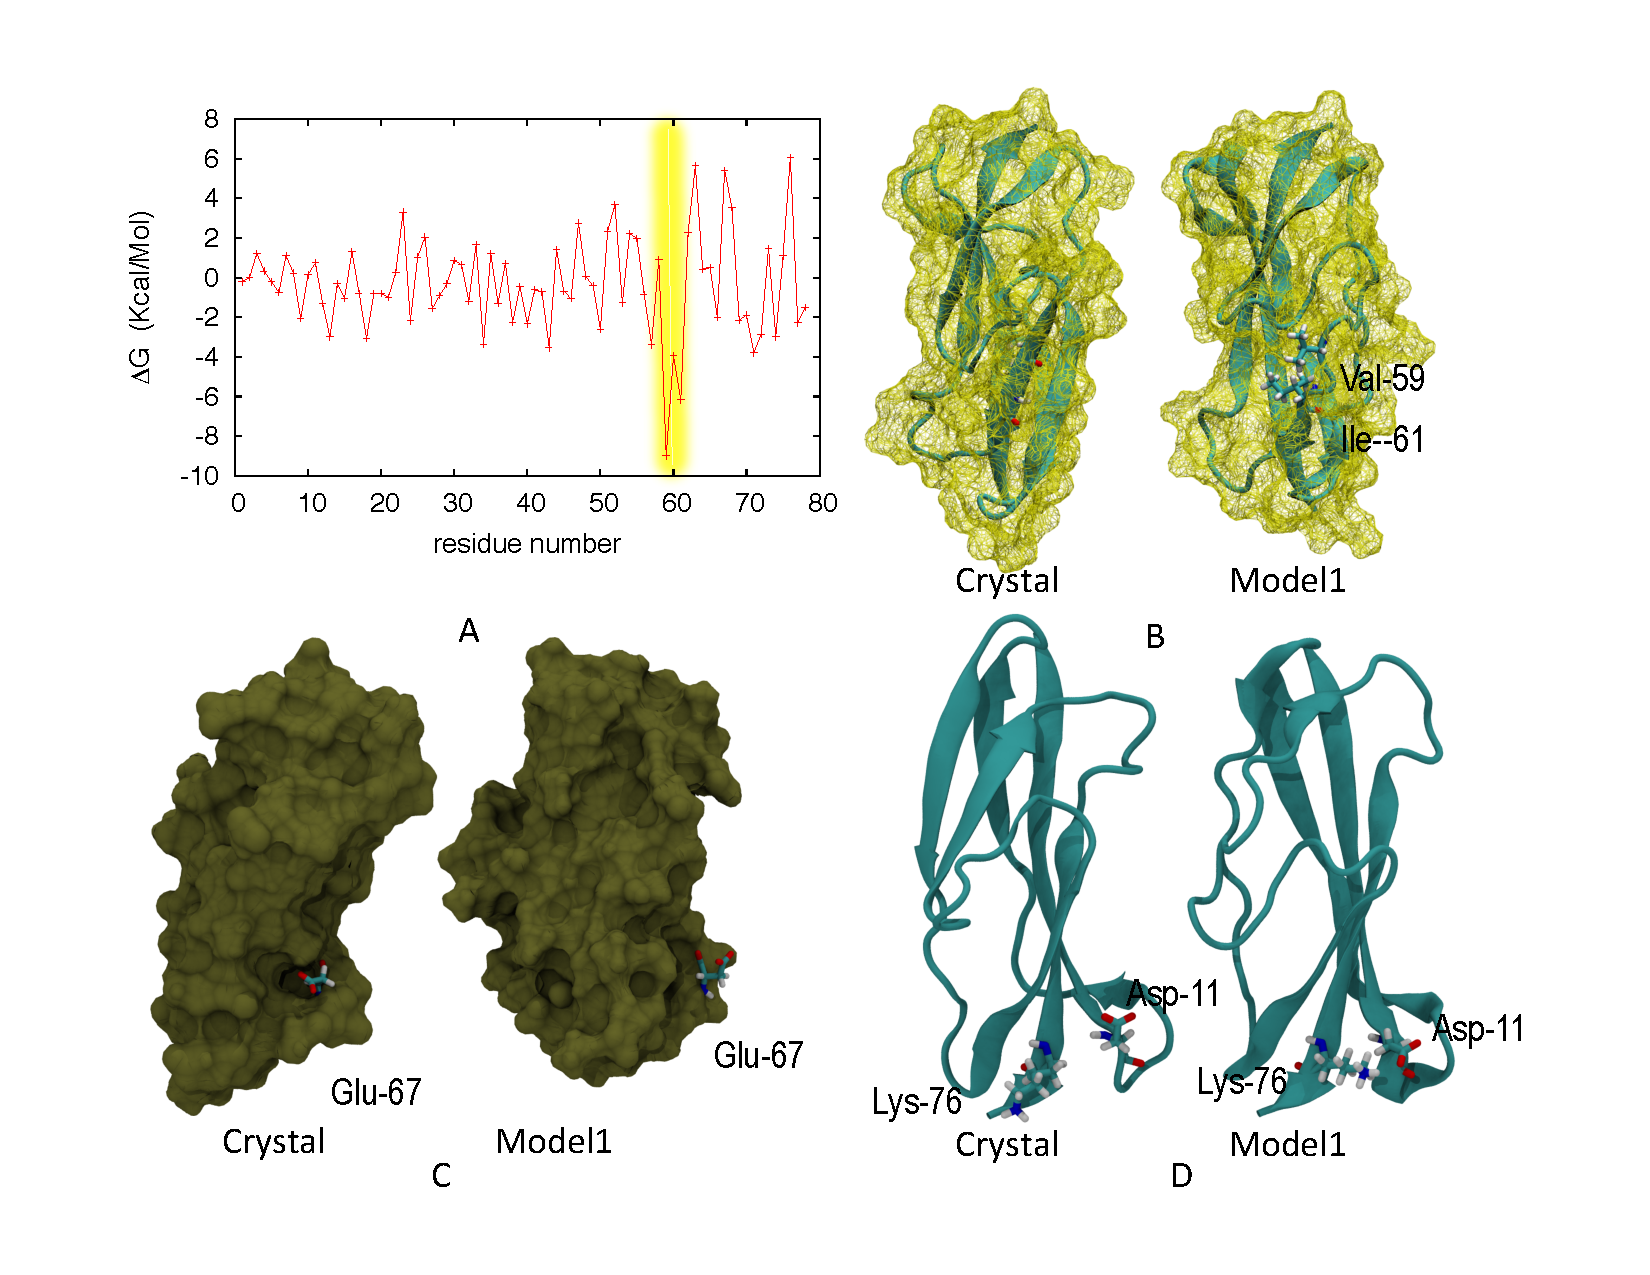
\includegraphics[width=5 in,height=4 in]{Target_569_per_residue.pdf}
\end{center}
\caption{A. Plot of per residue free energy difference between the model and the crystal structure of Traget 569 (pdb id: 2KWY) of CASP9.
B. In model 1, the beta sheet containing Val-59 and Ile-61 is disordered. These hydrophobic residues are exposed to the solvent.
C. Glu-67 is partially exposed to the solvent in crystal and it is fully exposed in model 1.
D. There is a H-bond between Lys-76 and Asp-11 in model 1, which is absent in the crystallaographic structure.}
\label{fig:T0569_per_residue}
\end{figure}


%\begin{figure}
%\begin{center}
%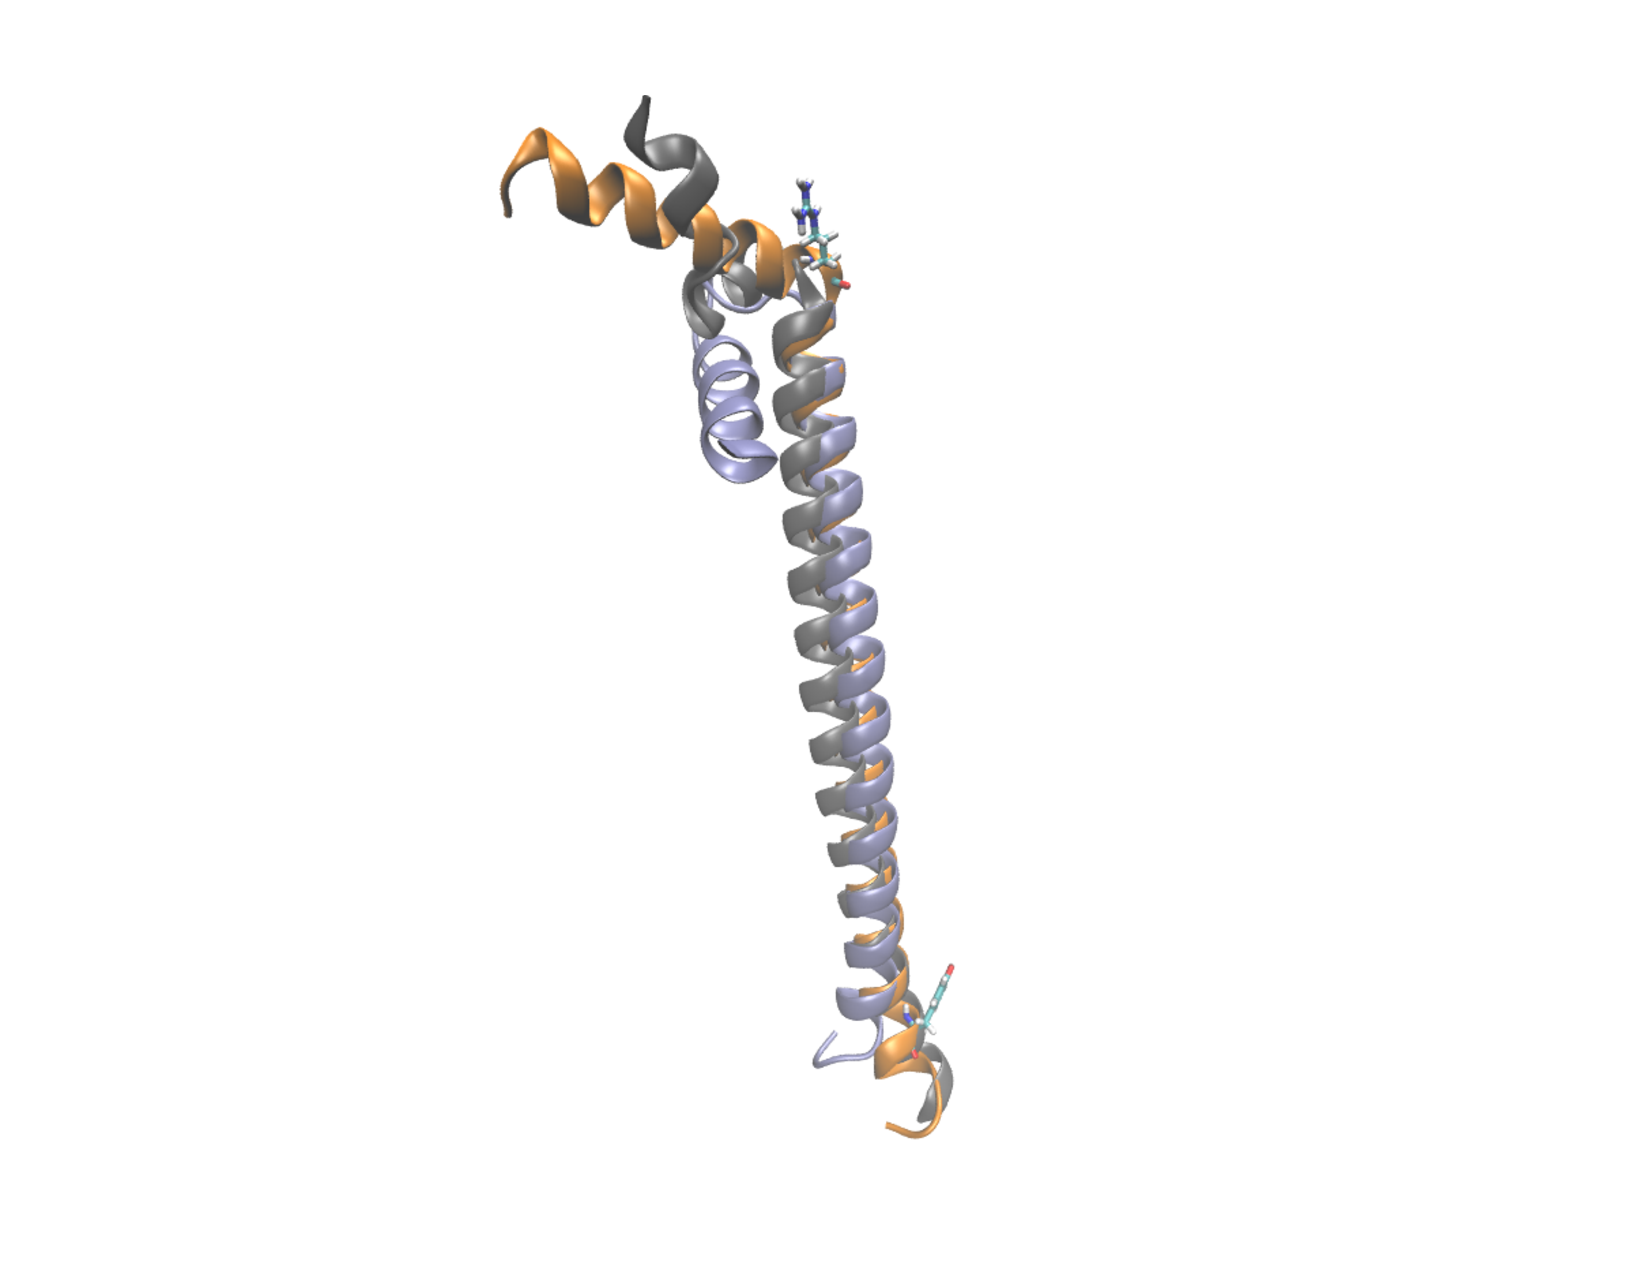
\includegraphics[width=12cm,height=10cm]{T0605.pdf}
%\end{center}
%\caption{ Three models of the leucine zipper domain of cGMP dependent protein
%kinase I (original pdb id: 3NMD and CASP target: T0605). The original target sequence of this protein was 72 residues.
%However only residues 3 to 66 is only kept during result announcement as that part can be found from crystallographic analysis. The
%region 3 to 66 are almost identical in all the 3 models  }
%\label{fig:T0605}
%\end{figure}


\begin{thebibliography}{99}

\bibitem{Meirovitch2007}
Meirovitch, H. Recent developments in methodologies for calculating the entropy and free energy of biological systems by computer simulation.
Current Opinion in Structural Biology, 2007, 17, 181-186.

\bibitem{Chipot2007}
Chipot, C.; Shell, M.S.; Pohorille, A. Introduction, in Chipot, C., Pohorille, A., editors. Free Energy
Calculations: Theory and Applications in Chemistry and Biology. Springer Series in Chemical
Physics, vol. 86. Berlin and Heidelberg: Springer; 2007, p. 1–32.

\bibitem{Jorgensen2004}
Jorgensen, W.L. The many roles of computation in drug discovery, Science 2004, 303, 1813–8.

\bibitem{Gilson2007}
Gilson, M.K.; Zhou, H.X. Calculation of protein-ligand binding affinities. Annu Rev Biophys Biomol Struct. (2007) 36, 21-42.

\bibitem{Torrie1977}
Torrie, G. M.; Valleau, J. P. iNonphysical sampling distributions in Monte Carlo free-energy estimation: Umbrella sampling 
(1977) J. Comput. Phys. 23, 187

\bibitem{Tironi1994}
Tironi, I.G.; van Gunsteren, W.F. A molecular-dynamics simulation study of chloroform. Mol. Phys. (1994) 83, 381-403.

\bibitem{Dill1997}
Dill, K.A.; H.S. Chan.  From Levinthal to Pathways to Funnels:  The "New View" of Protein Folding Kinetics.  Nature Structural Biology 4, 10-19 (1997)

\bibitem{Dill2008}
Dill, K.A.; Ozkan, S.B.; Shell, M.S.; Weikl, T.R. The protein folding problem. Annual Review of Biophysics (2008), 37, 289-316.

\bibitem{Anfinsen1973}
Anfinsen. C.B. Principles that Govern the Folding of Protein Chains. Science (1973) 181, 223-230.

\bibitem{Christ2007}
Christ, C.D.; van Gunsteren, W.F. Enveloping distribution sampling: A method to calculate free energy differences from a single simulation,
J. Chem. Phys. (2007), 126, 184110.

\bibitem{Ytreberg2006}
Ytreberg, F.; Zuckerman, D. Simple estimation of absolute free energies for biomolecules. J. Chem. Phys. 2006, 124, 104105.

\bibitem{Park2008}
Park, S.; Lau, A.; Roux, B. Computing conformational free energy by deactivated morphing. J. Chem. Phys. 2008, 129, 134102

\bibitem{Zheng2008}
Zheng, L.; Chen, M.; Yang, W. Random walk in orthogonal space to achieve efficient free-energy simulation of complex systems, Proc. Natl. Acad. Sci. 2008, 105 (51), 20227.

\bibitem{Tyka2006}
Tyka, M.; Clarke, A.; Sessions, R. An Efficient, Path-Independent Method for Free-Energy Calculations. J.Phys.Chem. B 2006, 110, 17212-17220.

\bibitem{Cecchini2009}
Cecchini, M., Krivov, S.V., Spichty, M., Karplus, M. Calculation of free-energy differences by confinement simulations. Application to peptide conformers. 
J. Phys. Chem. B 113, p. 9728-9740 (2009).

\bibitem{Strajbl2000}
Strajbl, M.; Sham, Y.Y.; Villà, J.; Chu, Z.-T.; Warshel, A. Calculations of Activation Entropies of Chemical Reactions 
in Solution. (2000) 104, 4578-4584.  

\bibitem{Krivov2004} 
Krivov, S.; Karplus, M. Hidden complexity of free energy surfaces for peptide (protein) folding Proc. Natl. Acad. Sci. U.S.A. 2004, 101, (41), 14766.

\bibitem{Alexander2007}
Alexander, P.A.; He, Y.; Chen, Y.; Orban, J. Bryan, P. The design and characterization of two proteins with $88 \%$ sequence identity but different 
structure and function. Proc. Natl. Acad. Sci. 2007, 104 (29), 11963-11968.

\bibitem{He2008}
He, Y.; Chen, Y.; Alexander, P.A.; Orban, J. NMR structures of two designed proteins with high sequence identity but different fold and function. Proc. Natl. Acad. Sci. 2008, 105 (38), 14412-14417.

\bibitem{Alexander2009}
Alexander, P.A.; He, Y.; Chen, Y.; Orban, J. Bryan, P. A minimal sequence code for switching protein structure and function. Proc. Natl. Acad. Sci. 2009, 106(50), 21149-21154.

\bibitem{Shortle20009}
Shortle, D. One sequence plus one mutation equals two folds. Proc. Natl. Acad. Sci. 2009, 106(50), 21011-21012. 

\bibitem{Sheffler2009}
Sheffler, W.; Baker, D. RosettaHoles: Rapid assessment of protein core packing for structure prediction, refinement, design, and validation. Protein Science. 2009, 18(1), 229-239.


\bibitem{MacCallum2011}
MacCallum, J.; Perez, A.; Schnieders, MJ.; Hua, L.; Jacobson, M.P.; Dill, K.A. Assessment of protein structure refinement 
in CASP9. Proteins, 2011, 79, 74-90.

\bibitem{Kryshtafovych2011}
Kryshtafovych, A.; Fidelis, K; and Tramontano, A. Evaluation of model quality predictions in CASP9. Proteins, 2011, 79, 91–106

\bibitem{Zemla2003}
Zemla, A. LGA: a method for finding 3D similarities in protein structures. Nucleic Acids Res 2003, 31, 3370–3374.


\bibitem{Perez2012}
Perez, A.; Yang, Z.; Bahar, I.; Dill, K.A.; MacCallum, J.L.; FlexE: Using Elastic Network Models to Compare Models of Protein Structure. J. Chem. Theory Comput., 2012, 8, 3985-3991. 

\bibitem{Wang2011}
Wang, Q.; Vantasin, K.; Xu, D.; Shang, Y. MUFOLD-WQA: A new selective consensus method for quality assessment in protein structure prediction. 
Proteins, 2011, 79: 185–195. 

\bibitem{Case2005}
Case, D.A.; Cheatham, III, T.E.; Darden, T.; Gohlke, Luo, H.R.; Merz, Jr., K.M.;  Onufriev, A; Simmerling, C.; 
Wang, B.; R. Woods, R. The Amber biomolecular simulation programs. J. Computat. Chem. (20005) 26, 1668-1688.



\end{thebibliography}

\end{document}

